% =============================================================================
% Cross-Dataset External Validation of a Retinal Foundation Model for Diabetic
% Retinopathy Grading: Performance, Explainability, and Uncertainty
%
% Template: IEEEtran (two-column journal style). IEEEtran.cls ships with every
% standard TeX Live / MiKTeX install; else CTAN: https://ctan.org/pkg/ieeetran
% This layout suits IEEE J-BHI / IEEE Access / IEEE TMI. For a fast-turnaround
% MDPI venue (Diagnostics, Journal of Imaging), swap the class for mdpi.cls and
% move title/author/abstract/keywords into its macros; the body needs no change.
%
% Compile: pdflatex main_standalone && bibtex main_standalone
%          && pdflatex main_standalone && pdflatex main_standalone
% =============================================================================
\documentclass[journal]{IEEEtran}

\usepackage{graphicx}
\usepackage{booktabs}
\usepackage{array}
\usepackage{multirow}
\usepackage{amsmath}
\usepackage{amssymb}
\usepackage{xcolor}
\usepackage{tikz}
\usetikzlibrary{arrows.meta,positioning}
\usepackage[hidelinks]{hyperref}

% This paper is table/figure dense; loosen LaTeX's two-column float placement so
% the spanning table*/figure* floats do not pile up at the end.
\setcounter{topnumber}{3}
\setcounter{bottomnumber}{2}
\setcounter{totalnumber}{5}
\setcounter{dbltopnumber}{3}
\renewcommand{\topfraction}{0.9}
\renewcommand{\bottomfraction}{0.7}
\renewcommand{\textfraction}{0.07}
\renewcommand{\floatpagefraction}{0.7}
\renewcommand{\dbltopfraction}{0.9}
\renewcommand{\dblfloatpagefraction}{0.7}


% Layout safety: let long file paths in \texttt break after "_" and "/",
% and give TeX a little extra stretch before it lets a line run into the margin.
\let\origunderscore\_
\renewcommand{\_}{\origunderscore\allowbreak}
\setlength{\emergencystretch}{1.5em}

\begin{document}

\title{Cross-Dataset External Validation of a Retinal Foundation Model for
Diabetic Retinopathy Grading: Performance, Explainability, and Uncertainty}

\author{Pravin Raj E%
\thanks{P.\ R.\ E is an independent researcher (no institutional
affiliation). ORCID: \href{https://orcid.org/0009-0000-2975-1631}{0009-0000-2975-1631}.
Correspondence: \texttt{epravinraj0761@gmail.com}.}%
\thanks{This work received no external funding and used only publicly available
datasets, one gated pretrained checkpoint (RETFound), and a single consumer GPU.}}

\markboth{Preprint --- under review}%
{Pravin Raj E: Cross-Dataset External Validation of a Retinal Foundation Model for DR Grading}

\maketitle

\begin{abstract}
Retinal foundation models such as RETFound are expected to generalise better
than ImageNet-pretrained networks, but protocol-matched external validation for
diabetic retinopathy (DR) grading is scarce. We applied one preprocessing,
fine-tuning, and evaluation protocol to ImageNet-pretrained EfficientNet-B3
(primary baseline) and ResNet-50 and to RETFound (ViT-Large/16; linear probing
and full fine-tuning), trained them on APTOS~2019 ($n=3662$), and evaluated
them unchanged on Messidor-2 ($n=1744$; adjudicated reference standard) and a
$455$-image copy of IDRiD. The primary outcome was the quadratic-weighted kappa
(QWK). The confirmatory family was the paired difference in internal-to-external
QWK drop between each RETFound variant and EfficientNet-B3 on each external set
(four contrasts, Holm-adjusted). Internally, fully fine-tuned RETFound and
EfficientNet-B3 were indistinguishable (QWK $0.882$ vs.\ $0.876$; paired
difference $+0.006$, $95\%$ CI $-0.014$ to $0.029$). Every model degraded
externally, most on Messidor-2 (EfficientNet-B3 QWK $0.499$, drop $0.377$).
Fully fine-tuned RETFound generalised neither better nor measurably worse than the CNN:
its excess drop was $+0.018$ ($95\%$ CI $-0.024$ to $0.058$) on Messidor-2 and
$+0.022$ ($-0.033$ to $0.083$) on IDRiD (Holm $p=0.79$ for both). The
RETFound linear probe degraded more than the CNN on both sets ($+0.076$, $0.019$
to $0.132$, Holm $p=0.030$; $+0.105$, $0.038$ to $0.170$, Holm $p=0.016$). In
secondary analyses the CNN had a higher referable-DR AUC than fully fine-tuned
RETFound on IDRiD ($0.962$ vs.\ $0.885$; DeLong $p<0.001$); RETFound's
label-smoothed probabilities were better calibrated externally (ECE
$0.09$--$0.13$ vs.\ $0.26$--$0.29$); single-pass softmax entropy was a weak
external error signal for every model (AUROC $0.49$--$0.68$) and carried none for
fully fine-tuned RETFound on IDRiD; and a geometric saliency-location proxy, not
a lesion-level assessment, placed RETFound's saliency on the image border more
often than the CNN's on Messidor-2. In this retrospective study of public
datasets, retinal-domain pretraining gave no measurable robustness advantage
over a standard ImageNet CNN on these shifts, and the external performance of
every model falls far short of what clinical use would require.
\end{abstract}

\begin{IEEEkeywords}
Diabetic retinopathy, retinal foundation models, RETFound, external validation,
domain shift, quadratic-weighted kappa, explainability, uncertainty
quantification, retinal imaging.
\end{IEEEkeywords}

\IEEEpeerreviewmaketitle


\section{Introduction}
\label{sec:intro}

Diabetic retinopathy (DR) is a leading cause of preventable vision loss, and the
number of people who need regular retinal screening grows faster than the number
of graders able to read their photographs. Automated grading of colour fundus
photographs is the obvious response, and supervised deep networks have reached
specialist-level agreement on the data they were developed on
\cite{gulshan2016,ting2017}. The difficulty begins when such a model meets
images it was not built for. Performance has repeatedly fallen when cameras,
populations, image quality, or the grading protocol change
\cite{beede2020,dai2021spectrum}, and reviews of DR screening AI note that
external validation, the test that would reveal this, is still reported
inconsistently \cite{grzybowski2020review,tripodai2024}.

Self-supervised foundation models are often presented as the answer to this
fragility. RETFound \cite{zhou2023retfound}, a Vision Transformer
\cite{dosovitskiy2021vit} pretrained with masked autoencoding \cite{he2022mae} on
about $1.6$~million unlabelled retinal images, is the best-known example for
fundus photographs. The intuition is appealing: a representation learned from
many retinas, rather than from ImageNet's everyday objects, should capture
retinal structure that survives a change of camera or clinic. RETFound was
reported to transfer well to several ocular and systemic tasks
\cite{zhou2023retfound}. Whether that intuition holds for DR grading under
dataset shift has been tested less directly. Hou et al.\ \cite{hou2025dinov2}
fine-tuned RETFound and a natural-image foundation model (DINOv2) on the same
three public DR datasets used here and evaluated them across datasets; the
natural-image model generally had the higher AUC. Other recent DR studies have
paired external validation with lesion-level evidence
\cite{jafarpoor2026multitask} or with uncertainty estimates
\cite{saleem2026cgdrnet}, but for supervised architectures rather than a retinal
foundation model.

Three things are therefore still unresolved. First, it is not established
whether retinal-domain pretraining makes DR \emph{grading} more robust than the
standard alternative that most deployed systems still use --- a supervised,
ImageNet-pretrained convolutional network --- when both are trained, tuned, and
evaluated in exactly the same way. Comparisons between foundation models, or
between models trained under different recipes, cannot answer this. Second, the
quantity that matters for robustness is not a model's external score but how much
it \emph{loses} between internal and external data, and whether that loss
differs between models by more than chance; this difference is rarely the
pre-specified estimand. Third, when a model does degrade, it matters whether its
own confidence warns the user. A model that fails while appearing uncertain is
far less dangerous than one that fails confidently. The answers matter in
practice: if retinal pretraining does not buy robustness, then choosing a
foundation model is not a substitute for external validation, and internal
parity between architectures says little about how they will behave elsewhere.

We address these gaps with a matched cross-dataset comparison. One preprocessing
pipeline, one fine-tuning protocol, one evaluation protocol, and one statistical
treatment were applied to RETFound (as a frozen linear probe and fully
fine-tuned) and to ImageNet-pretrained EfficientNet-B3 (primary baseline) and
ResNet-50. All models were developed only on APTOS~2019 and then scored once,
unchanged, on Messidor-2, whose labels are an adjudicated expert consensus, and
on IDRiD, which differs most in camera, resolution, and disease mix. We ask three
questions:
\begin{itemize}
  \item \textbf{RQ1 (Performance; primary).} Does RETFound lose less five-class
    grading agreement (quadratic-weighted kappa, QWK) between internal and
    external data than an ImageNet-pretrained CNN trained identically?
  \item \textbf{RQ2 (Uncertainty).} When the models err on external images, does
    their predictive uncertainty separate errors from correct predictions well
    enough to support referral of uncertain cases, and are their probabilities
    calibrated?
  \item \textbf{RQ3 (Explainability; exploratory).} Does each model's saliency
    on external images fall in the retinal region where DR lesions can occur,
    rather than on the optic disc or the image border? (Planned as a
    lesion-plausibility question; without lesion masks or blinded expert raters
    it can be answered here only by a geometric location proxy,
    Section~\ref{sec:methods-explain}.)
\end{itemize}

\textbf{What we found, in brief.} Fully fine-tuned RETFound and the CNN were
indistinguishable internally, and RETFound neither generalised better nor
measurably worse externally; used as a frozen feature extractor, RETFound
generalised worse. Every model lost much of its agreement on Messidor-2, and
uncertainty did not reliably flag the errors. The study also contains a
cautionary episode: an earlier, hardware-interrupted training run had suggested
that RETFound generalised significantly worse, and the difference vanished once
the pre-specified protocol was run to completion (Section~\ref{sec:discussion}).

\textbf{Contributions.} (i) A protocol-matched comparison of a retinal foundation
model with ImageNet CNNs on external DR grading, in which the inferential target
is a pre-specified, multiplicity-controlled family of paired differences in
internal-to-external QWK drop (Section~\ref{sec:methods-stats}); (ii) analyses of
whether each model's uncertainty, calibration, and saliency location remain
informative under shift; (iii) an audit of the public dataset copies against
their canonical releases, including a previously undocumented label discrepancy in
a widely shared IDRiD mirror (Section~\ref{sec:methods-idrid}); and (iv) a
release of code, split lists, per-image predictions, checkpoint hashes, and an
exact environment lock (Section~\ref{sec:repro}).

\textbf{Scope.} This is a retrospective study on public benchmark images. We
compare \emph{one} retinal foundation-model checkpoint (RETFound MAE,
colour-fundus weights) with ImageNet CNNs on \emph{one} task (five-class DR
grading). Nothing here is a prospective, clinical, or reader-study result, and
the conclusions should not be extended to other foundation models or tasks
without direct testing.

\begin{figure*}[!t]
\centering
\footnotesize
\resizebox{\textwidth}{!}{%
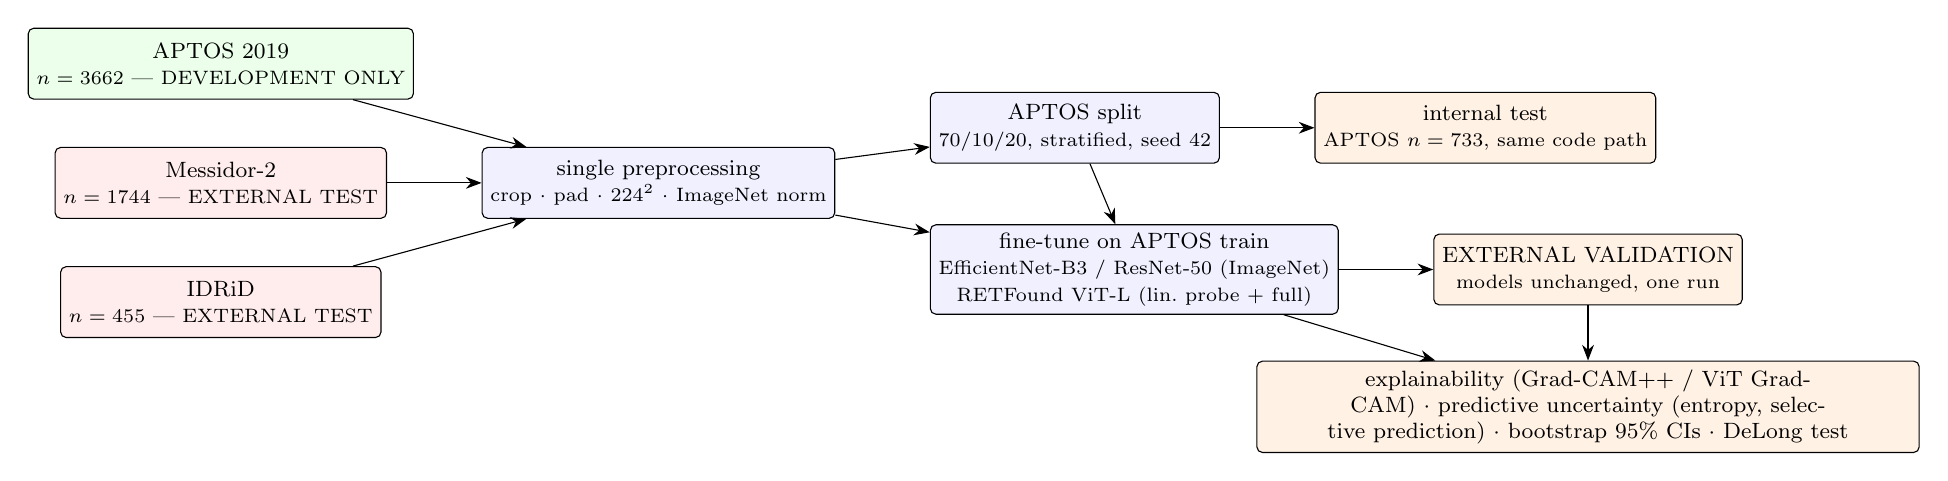
\begin{tikzpicture}[
  node distance=3.4mm and 6mm,
  box/.style={draw, rounded corners=2pt, align=center, inner sep=3pt, minimum height=9mm, font=\footnotesize},
  dev/.style={box, fill=green!8},
  ext/.style={box, fill=red!7},
  proc/.style={box, fill=blue!6},
  eval/.style={box, fill=orange!10},
  >={Stealth[length=2mm]}]
\node[dev] (aptos) {APTOS 2019\\{\scriptsize $n=3662$ --- DEVELOPMENT ONLY}};
\node[ext, below=6mm of aptos] (mess) {Messidor-2\\{\scriptsize $n=1744$ --- EXTERNAL TEST}};
\node[ext, below=6mm of mess] (idrid) {IDRiD\\{\scriptsize $n=455$ --- EXTERNAL TEST}};
\node[proc, right=12mm of mess] (pre) {single preprocessing\\{\scriptsize crop $\cdot$ pad $\cdot$ $224^2$ $\cdot$ ImageNet norm}};
\node[proc, right=12mm of pre, yshift=7mm] (split) {APTOS split\\{\scriptsize 70/10/20, stratified, seed 42}};
\node[proc, right=12mm of pre, yshift=-11mm] (ft) {fine-tune on APTOS train\\{\scriptsize EfficientNet-B3 / ResNet-50 (ImageNet)}\\{\scriptsize RETFound ViT-L (lin.\ probe + full)}};
\node[eval, right=12mm of split] (int) {internal test\\{\scriptsize APTOS $n=733$, same code path}};
\node[eval, right=12mm of ft] (extv) {EXTERNAL VALIDATION\\{\scriptsize models unchanged, one run}};
\node[eval, below=7mm of extv, text width=82mm] (an)
 {explainability (Grad-CAM++ / ViT Grad-CAM) $\cdot$ predictive uncertainty
  (entropy, selective prediction) $\cdot$ bootstrap $95\%$ CIs $\cdot$ DeLong test};
\draw[->] (aptos) -- (pre);
\draw[->] (mess) -- (pre);
\draw[->] (idrid) -- (pre);
\draw[->] (pre) -- (split);
\draw[->] (pre) -- (ft);
\draw[->] (split) -- (ft);
\draw[->] (split) -- (int);
\draw[->] (ft) -- (extv);
\draw[->] (ft) -- (an);
\draw[->] (extv) -- (an);
\end{tikzpicture}%
}
\caption{Study design. APTOS~2019 is used only for development (stratified
$70/10/20$ split); Messidor-2 and IDRiD are held out and opened once, for every
model, at external validation. One preprocessing pipeline, one fine-tuning
protocol, and one evaluation protocol are applied identically to the
ImageNet-pretrained CNNs and to RETFound.}
\label{fig:pipeline}
\end{figure*}


\section{Background and positioning}
\label{sec:related}

\textbf{Where external DR evaluation stands.} Large supervised DR systems
\cite{gulshan2016,ting2017} and a system spanning the full disease spectrum
\cite{dai2021spectrum} established high performance on their own data;
human-centred evaluation of a deployed system showed how poorly curated-test
performance predicted clinical behaviour \cite{beede2020}; and reviews flag
generalisation and external validation as under-reported
\cite{grzybowski2020review}. Recent external-validation studies have begun to
report lesion-level evidence \cite{jafarpoor2026multitask} and calibrated
uncertainty \cite{saleem2026cgdrnet} alongside grading accuracy, but for
supervised architectures.

\textbf{Retinal foundation models.} RETFound \cite{zhou2023retfound} adapts
masked-autoencoder pretraining \cite{he2022mae} to a ViT-Large
\cite{dosovitskiy2021vit} on large unlabelled retinal collections (about
$1.6$\,M colour fundus and OCT images in total; we use the colour-fundus
checkpoint). The closest prior work, Hou et al.\ \cite{hou2025dinov2}, compared
RETFound with DINOv2 on APTOS~2019, IDRiD, and Messidor-2, including
cross-dataset testing, and reported AUC; the natural-image model generally scored
higher on DR. That study compared two foundation models. It did not compare
RETFound with a supervised ImageNet CNN under one protocol, nor take the
internal-to-external drop in an ordinal grading metric as the estimand, nor ask
whether uncertainty flags external errors --- the three questions posed here.

\textbf{Positioning.} We make no claim of being first to externally validate DR
AI or to evaluate RETFound. The contribution is a specific, reproducible
combination: one foundation model and two ImageNet CNNs under a matched
preprocessing, fine-tuning, and evaluation protocol, with the paired difference
in internal-to-external QWK drop as a multiplicity-controlled primary estimand,
plus matched analyses of uncertainty, calibration, and saliency location, and a
full release. ResNet-50 \cite{he2016resnet} and EfficientNet-B3
\cite{tan2019efficientnet} were chosen as baselines because ImageNet-pretrained
CNNs of this kind are the usual reference point for pretrained representations in
medical imaging.


\section{Materials and Methods}
\label{sec:methods}

This study followed the TRIPOD+AI reporting guideline \cite{tripodai2024}; the
completed checklist is provided as supplementary material
(\texttt{paper/\allowbreak{}TRIPOD-AI\_checklist.md}). Figure~\ref{fig:pipeline} summarises the
design: freeze the datasets into development and external roles, apply one
preprocessing pipeline, fine-tune every model on APTOS only, and evaluate once
externally with a common resampling-based statistical treatment.

\subsection{Datasets}
\label{sec:methods-data}

Three public datasets were used (Table~\ref{tab:datasets};
Figure~\ref{fig:grades}). All three were downloaded and extracted on
2026-09-08 (the file-system date of every raw image and label file), which is
taken as the access date. Source, version, licence, and the full audit of each
local copy against its canonical release are in \texttt{DATA\_PROVENANCE.md}.

\begin{itemize}
  \item \textbf{APTOS 2019 Blindness Detection} \cite{aptos2019}: the $3662$
    labelled images of the Kaggle competition release (Aravind Eye Hospital,
    India; gathered from multiple clinics and cameras). The unlabelled $1928$-image
    Kaggle holdout was not used. Licence: Kaggle competition rules
    (non-commercial research; no redistribution). Used \emph{only} for model
    development (training, validation, internal test).
  \item \textbf{Messidor-2} \cite{decenciere2014,abramoff2013}: the canonical
    ADCIS release has $874$ examinations, each two macula-centred images (one
    per eye), $1748$ images in total. We used the $1744$ images graded
    gradable under the adjudicated reference standard of Krause et
    al.\ \cite{krause2018}; the four absent images are exactly those marked
    ungradable. Licence: ADCIS terms (research and education; no
    redistribution). External test only.
  \item \textbf{IDRiD} (Disease-Grading subset) \cite{porwal2018,porwal2020}:
    the official IEEE DataPort release (doi:10.21227/H25W98, CC~BY~4.0) has
    $516$ images ($413$ train $+$ $103$ test). The copy used here, a third-party
    Kaggle mirror, contains $455$ of them ($375$ train IDs, $80$ test IDs);
    Section~\ref{sec:methods-idrid} characterises the $61$ missing images and a
    label discrepancy found in the mirror. External test only; both official
    IDRiD splits were pooled because neither was used for training.
\end{itemize}

\subsubsection{Audit of the IDRiD copy}
\label{sec:methods-idrid}
The $61$ missing images ($38$ train IDs, $23$ test IDs; listed in
\texttt{data\_splits/\allowbreak{}idrid\_missing\_vs\_official.csv}) fall mostly in
contiguous ID runs ($22$ of the $38$ train IDs lie in 138--173), which suggests
an incomplete upload rather than selection by grade, although the cause cannot
be established. Against the official per-grade counts ($168/25/168/93/62$ for
grades 0--4), the mirror's $129/22/156/84/64$ under-represents grade~0
($28.4\%$ vs.\ $32.6\%$) and raises the referable-DR prevalence from $62.6\%$ to
$66.8\%$. The mirror also holds more grade-4 images among the official
\emph{train} IDs ($55$) than the official train set contains ($49$), and more
grade-3 images among the test IDs ($20$ vs.\ $19$); removing images cannot
produce this, so at least $7$ of the $455$ mirror labels ($\geq 1.5\%$) differ
from the official grades. The exact number cannot be determined without the
official per-image label file. To bound the effect of the class-mix
difference we re-weighted the $455$ images by grade to the official $516$-image
mix (Section~\ref{sec:methods-stats}); the label discrepancy is a separate,
stated limitation (Section~\ref{sec:limitations}).

\subsubsection{Reference standards and their comparability}
\label{sec:methods-refstd}
The three reference standards were produced differently. APTOS labels were
assigned by one clinician per image on a 0--4 scale; no second reading or
adjudication is described \cite{aptos2019}. Messidor-2 labels are the
adjudicated consensus of three fellowship-trained retina specialists who graded
independently on the ICDR scale and resolved every disagreement in adjudication
sessions \cite{krause2018}. IDRiD labels were assigned by ``medical experts''
on a 0--4 scale based on the ICDR scale; the number of graders and any
adjudication are not reported \cite{porwal2018}. An internal-to-external QWK drop
therefore combines image-domain shift with a change of labelling protocol, and
QWK values are not directly comparable \emph{across} the two external datasets.
Because every model is scored against the same labels on the same images, this
protocol difference does not by itself favour either model in the
between-model contrasts that form the primary inference
(Section~\ref{sec:methods-stats}), but it does limit how much of each model's
absolute drop can be attributed to the images.

Messidor-2 and IDRiD were not used for any modelling, hyperparameter,
checkpoint, or threshold decision (Section~\ref{sec:methods-lock}).

\begin{table}[!t]
\centering\small
\caption{Dataset characteristics. Grade share is the percentage of gradable
images at each ICDR severity level. See Figure~\ref{fig:grades} for a visual
comparison.}
\label{tab:datasets}
\setlength{\tabcolsep}{3pt}
\begin{tabular}{lrlc}
\toprule
Dataset & $n$ & Role & Grades 0/1/2/3/4 (\%) \\
\midrule
APTOS 2019 & $3662$ & Development   & 49.3/10.1/27.3/5.3/8.1 \\
Messidor-2 & $1744$ & External test & 58.3/15.5/19.9/4.3/2.0 \\
IDRiD      & $455$  & External test & 28.4/4.8/34.3/18.5/14.1 \\
\bottomrule
\end{tabular}
\end{table}

\begin{figure}[!t]
\centering
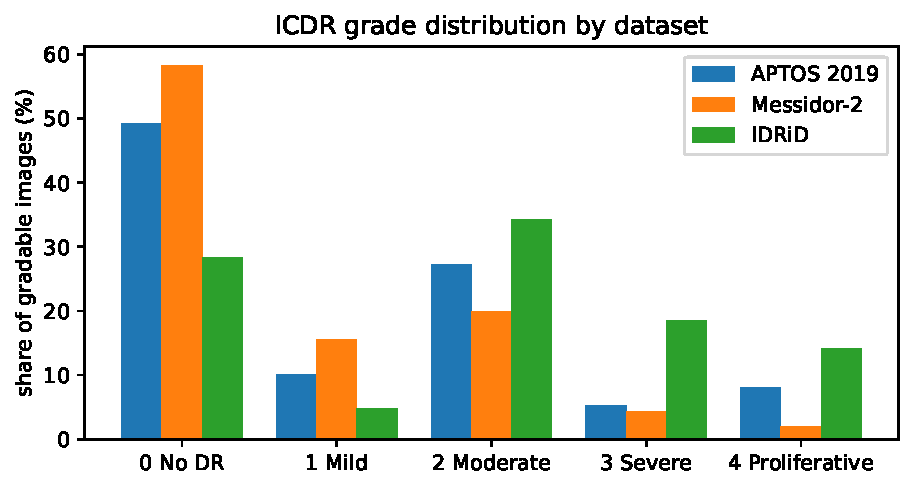
\includegraphics[width=\linewidth,height=0.30\textheight,keepaspectratio]{figures/fig_grades.pdf}
\caption{ICDR grade distribution by dataset. APTOS and Messidor-2 are
grade-0-dominated; IDRiD is pathology-enriched (modal grade 2), which shapes the
interpretation of its internal-to-external drop
(Section~\ref{sec:results-ext}).}
\label{fig:grades}
\end{figure}

\subsection{Domain-shift characterisation}
\label{sec:methods-shift}

Table~\ref{tab:shift} contrasts the three datasets on the acquisition and
labelling axes that plausibly drive the external drop: country and population,
camera and mydriasis, native resolution and field of view, illumination/colour
uniformity, image quality, DR-grade prevalence, and the reference standard. The
two external sets differ from APTOS in complementary ways: Messidor-2 shares the
$\approx$45$^\circ$ macula-centred geometry and has a \emph{lower} referable-DR
prevalence but a stricter, adjudicated-consensus reference standard, whereas IDRiD
differs most on resolution, mydriasis, and prevalence (referable-DR $66.8\%$ in
the copy used here versus $40.6\%$ in APTOS). Section~\ref{sec:results-ext} interprets the two
failure modes against this table.

\begin{table*}[!t]
\centering\footnotesize
\caption{Domain-shift characterisation of the three datasets, compiled from the
dataset publications, the release pages, and \texttt{DATA\_PROVENANCE.md}.
``Reference standard'' is the labelling process; prevalences are computed from
the copies used in this study (IDRiD: $455$-image copy).}
\label{tab:shift}
\setlength{\tabcolsep}{4pt}
\begin{tabular}{@{}>{\raggedright\arraybackslash}p{0.17\textwidth} >{\raggedright\arraybackslash}p{0.25\textwidth} >{\raggedright\arraybackslash}p{0.25\textwidth} >{\raggedright\arraybackslash}p{0.25\textwidth}@{}}
\toprule
Axis & APTOS 2019 (development) & Messidor-2 (external) & IDRiD (external) \\
\midrule
Country / population & India, Aravind Eye Hospital; multiple clinics & France: Messidor programme partners (Original) and Brest University Hospital (Extension) & India, Eye Clinic, Nanded, Maharashtra \\
Camera & multiple, not individually published & Extension: Topcon TRC NW6; Original: not stated in the release & Kowa VX-10$\alpha$ \\
Mydriasis & not published & Extension: none; Original: not stated in the release & all dilated (tropicamide $0.5\%$) \\
Native resolution & heterogeneous, $\approx$1.5--3\,MP & 1440$\times$960 to 2304$\times$1536 & 4288$\times$2848 \\
Field of view & $\approx$45$^\circ$, macula-centred & $\approx$45$^\circ$, macula-centred & 50$^\circ$, macula-centred \\
Illumination / colour & variable across sites & more uniform & high, uniform \\
Image quality & variable; low-quality frames retained & ungradable images excluded (4 of 1748) & high and uniform \\
Images per patient & unknown (no patient IDs) & 2 per examination (one per eye) & unknown (no patient IDs) \\
Grade prevalence 0/1/2/3/4 (\%) & 49.3 / 10.1 / 27.3 / 5.3 / 8.1 & 58.3 / 15.5 / 19.9 / 4.3 / 2.0 & 28.4 / 4.8 / 34.3 / 18.5 / 14.1 \\
Referable DR ($\geq 2$), \% & 40.6 & 26.2 & 66.8 (official release: 62.6) \\
Reference standard & one clinician per image; no adjudication described & \textbf{adjudicated consensus of 3 retina specialists} \cite{krause2018} & ``medical experts''; number of graders and adjudication not reported \\
\bottomrule
\end{tabular}
\end{table*}

\subsection{Preprocessing}
\label{sec:methods-pre}

A single preprocessing script was applied identically to all three datasets:
(i) conversion to RGB; (ii) tolerance-based cropping of the black frame around the
circular fundus; (iii) zero-padding to a centred square (aspect ratio preserved);
(iv) bilinear resizing to $224\times224$ (RETFound's native input). Channel
normalisation used ImageNet statistics
($\mu=(0.485,0.456,0.406)$, $\sigma=(0.229,0.224,0.225)$), consistent with
RETFound's downstream configuration. Contrast-limited adaptive histogram
equalisation was implemented as an optional step and was \emph{not} applied in the
primary analysis. Messidor-2's mirror mixes vendor-preprocessed and original
frames in one folder; the single pipeline was applied to all $1744$ images
regardless of source form. All $5861$ preprocessed images passed a stratified
visual audit for label--image alignment.

\subsection{Development split}
\label{sec:methods-split}

APTOS~2019 was partitioned $70\%/10\%/20\%$ into training, internal validation,
and internal test, stratified by DR grade, with a fixed random seed ($42$); the
exact image-ID lists are released
(\texttt{data\_splits/\allowbreak{}aptos\_\{train,val,test\}.csv}). Table~\ref{tab:counts}
gives the per-split, per-grade image counts.

\textbf{Duplicate / leakage check.} A byte-level (MD5) check of all $5861$
preprocessed images (\texttt{scripts/\allowbreak{}phase12\_leakage.py}) found \emph{no}
exact-duplicate image shared between any two of the three datasets: Messidor-2 and
IDRiD contain no byte-copy of an APTOS image or of each other, so the external
validation is uncontaminated. Within APTOS, which is known to contain repeated
images, $41$ of the $733$ internal-test images ($5.6\%$) have an exact duplicate
in the training or validation split. Removing them changes the internal-test QWK
by $+0.001$ to $+0.006$ and accuracy by $+0.007$ to $+0.013$ for every model (the
duplicated images were slightly harder than average, so the leakage marginally
\emph{understates} internal performance rather than inflating it); the direction
of every internal comparison is unchanged
(\texttt{outputs/\allowbreak{}phase12/\allowbreak{}dedup\_internal\_metrics.csv}). All external numbers,
which are the paper's focus, are unaffected. A semantic near-duplicate check
(ImageNet-pretrained EfficientNet-B3 features, $1536$-d, cosine similarity over
all cross-dataset image pairs; \texttt{scripts/\allowbreak{}phase14\_embedding\_dedup.py})
supports the byte-level result: no cross-dataset pair exceeded cosine $0.965$ and
none reached $0.98$, with no cluster near $1.0$, i.e.\ no evidence of
semantically duplicated images across datasets
(\texttt{outputs/\allowbreak{}phase14/\allowbreak{}}).

\textbf{Patient- and eye-level linkage.} None of the three releases provides a
patient identifier. APTOS image IDs are opaque hashes with no patient, eye, or
visit field, so the APTOS split is image-level, and both eyes or repeat images
of one patient can fall on both sides of it. The checks that were possible ---
the exact-duplicate check above and the deduplicated re-scoring --- bound only
the identical-image part of that risk; fellow-eye or repeat-visit images that
are not byte-identical cannot be detected, and the internal estimates may be
optimistic for that reason. This does not affect the external sets, which were
never used for training. Within Messidor-2, each examination contributes two
images (one per eye); the ADCIS pairing spreadsheet is not part of the copy used
here, so images could not be grouped by examination. IDRiD has no patient
identifiers. Image-level bootstrap intervals therefore treat possibly
correlated images as independent, and we report a worst-case sensitivity
analysis that halves the effective sample size of every test set
(Section~\ref{sec:methods-stats}).

\begin{table}[!t]
\centering\small
\caption{Image counts by split and ICDR grade. APTOS is split
$70/10/20$ stratified by grade (seed $42$); Messidor-2 and IDRiD are used whole
as external test sets.}
\label{tab:counts}
\setlength{\tabcolsep}{4pt}
\begin{tabular}{lrrrrrr}
\toprule
Split & $n$ & g0 & g1 & g2 & g3 & g4 \\
\midrule
APTOS train & 2562 & 1263 & 259 & 699 & 135 & 206 \\
APTOS validation & 367 & 181 & 37 & 100 & 19 & 30 \\
APTOS internal test & 733 & 361 & 74 & 200 & 39 & 59 \\
\midrule
Messidor-2 (external) & 1744 & 1017 & 270 & 347 & 75 & 35 \\
IDRiD (external) & 455 & 129 & 22 & 156 & 84 & 64 \\
\bottomrule
\end{tabular}
\end{table}

\subsection{Models and fine-tuning}
\label{sec:methods-models}

\textbf{Baseline CNN.} EfficientNet-B3 \cite{tan2019efficientnet} (primary) and
ResNet-50 \cite{he2016resnet} (secondary), ImageNet-pretrained
(\texttt{torchvision}), with the classifier head replaced by a five-way head.
Full fine-tuning (all layers unfrozen), AdamW ($\text{lr}=10^{-4}$, weight decay
$10^{-4}$), cosine annealing, batch size $32$, mixed precision, up to $30$ epochs
with early stopping on internal-validation QWK (patience $7$). The loss was
cross-entropy weighted by inverse class frequency. Augmentation:
horizontal/vertical flips, $\pm15^{\circ}$ rotation, mild brightness/contrast
jitter.

\textbf{RETFound.} The ViT-Large/16 masked-autoencoder checkpoint pretrained on
colour fundus images \cite{zhou2023retfound} was loaded (encoder weights only;
pretrained final LayerNorm reused as the pooling norm; fresh five-way head). Two
variants were fine-tuned, forming the principal ablation: (a) \emph{linear
probing} --- backbone frozen, head trained (base $\text{lr}=10^{-3}$, up to $40$
epochs); (b) \emph{full fine-tuning} --- all layers unfrozen with layer-wise
learning-rate decay ($0.65$), drop-path $0.2$, label smoothing $0.1$, base
$\text{lr}=10^{-4}$, batch size $16$, up to $30$ epochs. Data, normalisation,
class weighting, metric set, and early-stopping rule were identical to the
baseline. All hyperparameters are logged
(\texttt{outputs/\allowbreak{}phase\{4,5\}\_*/\allowbreak{}\,*\_hyperparams.json}).

\subsection{Evaluation metrics}
\label{sec:methods-metrics}

Given the marked class imbalance in every dataset, the primary metric was the
quadratic-weighted kappa (QWK) \cite{cohen1968kappa}, which credits ordinal
proximity. Secondary metrics: overall accuracy, macro-averaged F1, balanced
accuracy, per-class sensitivity and specificity, and one-vs-rest AUC (per class
and macro-averaged). The internal-to-external \emph{drop} in each metric is
reported per model per external dataset.

\subsection{External validation}
\label{sec:methods-ext}

Each trained model was run once, unmodified and without any further training or
threshold tuning, on Messidor-2 and on IDRiD, and re-scored on the APTOS internal
test set through the identical inference code path. Per-image outputs (true label,
predicted label, class probabilities, predictive entropy) were retained for all
model $\times$ dataset combinations.

\subsubsection{Locking the external evaluation}
\label{sec:methods-lock}
The external sets were kept out of every model decision, and the repository
history documents this. All training code and hyperparameter defaults were
committed before any external image was scored (CNN trainer 2026-09-08 12:28,
RETFound trainer 12:44; first external scoring, of the CNN baselines only,
13:16, local time) and were not changed afterwards: the git diff of both
trainers between their first commit and the commits that produced the frozen
checkpoints is empty, and later edits added only infrastructure options whose
defaults reproduce the original behaviour. Checkpoints were selected by APTOS
validation QWK alone; no threshold or temperature was fitted on external data.
Contact with external images before scoring was limited to the data audit
(counts, label parsing) and to running the already-fixed preprocessing with a
visual label--image alignment check. Analyses that scored external sets for
\emph{additional} configurations (inference-time ablations, seed and loss
sweeps, the head-depth sweep) came after the primary results and did not
replace any primary checkpoint. The completed RETFound full fine-tune
re-ran the identical pre-specified protocol; its only addition was
resume-from-last-epoch to survive hardware interruptions. The four frozen
checkpoints used for every primary comparison, every sensitivity-analysis
checkpoint, and their SHA-256 hashes are listed in \texttt{CHECKPOINTS.md};
the superseded interrupted-run checkpoint and its outputs are retained there for
comparison.

\subsection{Uncertainty quantification}
\label{sec:methods-unc}

\textbf{Primary measure.} Predictive uncertainty was the Shannon entropy of the
softmax output of a single deterministic forward pass (all stochastic layers in
evaluation mode). This is a point-estimate confidence score, not a Bayesian or
Monte-Carlo estimate.

\textbf{Sensitivity analysis (stochastic forward passes).} We repeated the
analysis with the entropy of the mean softmax over $T=20$ forward passes in
which the layers that were stochastic during training were kept active. What
those layers are differs by model, so the label ``Monte-Carlo dropout'' fits
only part of it: for the CNNs it is dropout before the classification head
(Monte-Carlo dropout in the sense of \cite{gal2016dropout}); for the RETFound
full fine-tune it is stochastic depth (drop-path, rate $0.2$) in the
transformer blocks, which randomly skips residual branches rather than dropping
units; and the RETFound linear probe has no stochastic layer in its trained
path, so its $T$-pass output equals its single-pass output. We call this the
\emph{stochastic-pass} analysis throughout. For
each model and external dataset we tested whether misclassified images carried
higher entropy than correctly classified images with a one-sided Mann--Whitney
$U$ test, reporting the rank-biserial correlation as the effect size, and we
computed the AUROC of predictive entropy used directly as a binary error
detector. We then plotted selective-prediction curves: images were ranked by
entropy and the most uncertain fraction referred out, and the accuracy,
quadratic-weighted kappa, and fraction of all errors captured among the referred
images were recorded as a function of retained coverage. Predictive entropy and
accuracy were also broken down by ICDR grade --- stratified both by the reference
grade and by the predicted grade --- to test whether a model reserved its
uncertainty for the rarer sight-threatening grades and whether the many grade-0
predictions it issued on the external sets were made confidently. Code:
\texttt{scripts/\allowbreak{}phase8\_uncertainty.py}, \texttt{scripts/\allowbreak{}phase8\_mc\_dropout.py}.

\subsection{Calibration}
\label{sec:methods-calib}

For each model and dataset (internal and external) we computed the expected
calibration error (ECE, $15$ equal-width confidence bins), the maximum
calibration error (MCE), the multi-class Brier score, and the negative
log-likelihood from the stored class probabilities, with a $95\%$ bootstrap CI on
ECE, and drew reliability diagrams
(\texttt{scripts/\allowbreak{}phase11\_review\_response.py}). Calibration is reported
separately for the internal APTOS test set and the two external sets. As a
recalibration check we also fitted a single scalar temperature per model by
minimising the negative log-likelihood on the APTOS \emph{validation} split
(used for early stopping, never for test or external scoring), applied that
temperature unchanged to the internal-test and both external sets, and recomputed
every calibration metric (\texttt{scripts/\allowbreak{}phase13\_temperature\_scaling.py}). The
fitted temperature was bootstrapped ($1000$ resamples) for a $95\%$ interval, and
the fit was repeated on a disjoint stratified subset of the APTOS training split
as a calibration-source robustness check. Temperature scaling is monotonic in the
logits, so it leaves accuracy and the quadratic-weighted kappa unchanged.

\subsection{Explainability}
\label{sec:methods-explain}

For a grade-stratified sample of correctly and incorrectly classified external
images (image identifiers drawn from the external-validation prediction files with
a fixed seed; forty correct and twenty-five incorrect per model per external
dataset, $65$ per cell), a saliency map was generated for the model's predicted
class. For the
convolutional networks this was a Grad-CAM++ map
\cite{chattopadhay2018gradcampp} at the last convolutional block; for the Vision
Transformer it was a method-matched Grad-CAM map at the last transformer block
(gradient-weighted patch-token activations for the predicted class, class token
removed, reshaped to the $14\times14$ patch grid and bilinearly upsampled).
Attention-rollout maps \cite{abnar2020rollout} were also computed but were more
diffuse and border-biased and are reported only in the supplement.

\textbf{What was and was not measured.} The study was planned to ask whether
saliency overlaps visible DR lesions. That requires lesion masks or blinded
expert grading, and neither was available: the IDRiD Disease-Grading subset has
no lesion masks, and no clinician rater was recruited. We therefore report only
a \emph{geometric location proxy}, and we make no claim about lesion focus or
clinical plausibility. A map was labelled \emph{in-zone} when its peak lay
inside the fundus, outside an automatically estimated optic-disc region and
outside an outer border annulus, and at least half of its top-decile saliency
mass lay in that same zone. The zone is where DR lesions \emph{can} occur, but it
also contains vessels, the macula, and normal retina, so an in-zone map can be
centred on vessels or on no pathology at all; conversely, the proxy is
informative mainly in the negative direction, when saliency falls on the border
annulus or the disc (Section~\ref{sec:limitations}). To make the planned expert
assessment executable without
re-deriving the sample, we additionally release a blinded rating packet
(\texttt{scripts/\allowbreak{}phase7\_rating\_packet.py}): $160$ maps ($10$ per model per
external dataset per correctness stratum, grade-stratified, seed $42$), each
re-rendered as a two-panel image (fundus and heatmap only, with no disc marker,
peak marker, or identifying text), a shuffled blind identifier, a rating sheet
and rubric, and a withheld key; the companion scorer computes the expert
lesion-focus rate, the expert-versus-proxy Cohen's $\kappa$, and the
inter-rater $\kappa$ per cell. It has not yet been completed by clinicians, so
no expert result is reported. Code:
\texttt{scripts/\allowbreak{}phase7\_explainability.py},
\texttt{scripts/\allowbreak{}phase7\_rating\_packet.py}.

\subsection{Statistical analysis}
\label{sec:methods-stats}

\textbf{Primary outcome and estimands.} QWK is the single primary outcome. For
each model and external dataset the estimand is the internal-to-external QWK
drop, and the inferential quantity is the \emph{difference} in that drop between
a comparator and the EfficientNet-B3 baseline ($\Delta$drop; positive $=$ the
comparator lost more ordinal agreement). We also report the paired difference in
QWK itself on each dataset (comparator minus baseline) as a descriptive
contrast. Every other metric (accuracy, macro-F1, balanced accuracy, AUC,
per-grade sensitivity and specificity, calibration, referable-DR operating
points) is secondary.

\textbf{Resampling.} Confidence intervals were obtained by non-parametric
bootstrap resampling of the relevant test set(s) with replacement ($2000$
iterations; NumPy PCG64 generator, seed $42$), recomputing each metric on every
resample and taking the $2.5$th and $97.5$th percentiles
\cite{efron1994bootstrap}. For a drop, the internal APTOS test set and the
external set were resampled independently within each iteration. For a
between-model contrast, the same resampled image indices were scored for both
models, so the contrast is paired at the image level. Two-sided bootstrap
$p$-values were obtained by percentile inversion,
$p=2\min\{\Pr^*(\hat\theta^*\leq 0),\Pr^*(\hat\theta^*\geq 0)\}$ with the
$(k+1)/(B+1)$ correction.

\textbf{Confirmatory family and multiplicity.} The confirmatory family is fixed
by the research question (RQ1) and has four members: $\Delta$drop for the
RETFound full fine-tune and for the RETFound linear probe, each against
EfficientNet-B3, on Messidor-2 and on IDRiD. Because a claim that RETFound
generalises worse (or better) could rest on any one of these four, we control
the family-wise error rate across them: we report Holm-adjusted $p$-values and,
alongside each $95\%$ CI, a Bonferroni-adjusted $98.75\%$ CI, and a
confirmatory claim is made only when the Holm-adjusted $p<0.05$. The ResNet-50
contrasts are a secondary comparison between two ImageNet CNNs and are not in
the family. The DeLong test \cite{delong1988,sun2014fast} on the referable-DR
binarisation (ICDR grade $\geq 2$; score $=$ summed probability of grades
2--4) is a secondary analysis; its nine comparisons (three comparators $\times$
three datasets) are reported with their own Holm adjustment
(\texttt{outputs/\allowbreak{}phase11/\allowbreak{}multiplicity.csv}). Per-grade
one-vs-rest DeLong tests, per-class sensitivities, calibration differences, and
all ablation and sensitivity analyses are exploratory: they are reported with
unadjusted CIs, are not used for confirmatory claims, and are labelled as
exploratory where they appear.

\textbf{Sensitivity analyses of the inference.} (i) \emph{Non-independent
images.} Because images could not be grouped by patient or examination
(Section~\ref{sec:methods-split}), we repeated every $\Delta$drop interval with
an $m$-out-of-$n$ bootstrap using $m=n/2$ on every test set, which is the
interval one would obtain if every image had a perfectly correlated partner
(e.g.\ the fellow eye; Messidor-2 has exactly two images per examination). (ii)
\emph{IDRiD missingness.} IDRiD QWK and $\Delta$drop were recomputed with each
image weighted by the ratio of its grade's share in the official $516$-image
release to its share in the $455$-image copy (Section~\ref{sec:methods-idrid}).
(iii) \emph{Stochastic passes.} The whole procedure was re-run on the $T=20$
stochastic-pass predictive distributions in place of the single forward pass
(\texttt{outputs/\allowbreak{}phase8/\allowbreak{}mc\_lp\_deterministic/}; the linear
probe, which has no training-time stochastic layer, enters with its single-pass
predictions).
Code: \texttt{scripts/\allowbreak{}phase9\_stats.py} (CIs, drops, DeLong),
\texttt{scripts/\allowbreak{}phase23\_primary\_inference.py} (confirmatory family,
Holm, paired QWK differences, sensitivity analyses (i)--(ii)),
\texttt{scripts/\allowbreak{}phase11\_review\_response.py} (calibration, per-class
CIs). Analyses used \texttt{numpy}, \texttt{pandas}, \texttt{scipy}, and
\texttt{scikit-learn} in Python~3.14.

Every headline number in Tables~\ref{tab:master}--\ref{tab:delong} was
independently recomputed from the released per-image prediction files with a
separate script (\texttt{scripts/\allowbreak{}phase11\_review\_response.py}); all $60$
recomputed metric cells matched the reported values to within $5\times10^{-4}$.

\subsection{Reproducibility}
\label{sec:methods-repro}

All code (preprocessing, split generation, training, evaluation, statistics), the
exact split image-ID lists, per-image prediction files, checkpoint identifiers
with SHA-256 hashes, the exact package lock of the environment, and the
TRIPOD+AI checklist are released (Section~\ref{sec:repro}). Raw images and the
pretrained RETFound weights are not redistributed, for licence reasons given in
Section~\ref{sec:repro}.


\section{Results}
\label{sec:results}

The results follow the three questions. We first establish that the models start
from comparable internal performance (Section~\ref{sec:results-int}), then answer
RQ1 with the primary outcome and test how robust that answer is
(Section~\ref{sec:results-ext}) and whether it holds for the binary referable-DR
decision (Section~\ref{sec:results-referable}). RQ2 asks whether the models'
uncertainty and probabilities remain informative once they err
(Sections~\ref{sec:results-unc}--\ref{sec:results-ood}). RQ3 and two exploratory
probes then ask where the models look and how sensitive they are to the input
distribution (Sections~\ref{sec:results-explain}--\ref{sec:results-headsummary}).

\subsection{Internal performance}
\label{sec:results-int}

On the APTOS internal test set ($n=733$; Table~\ref{tab:master}),
EfficientNet-B3 reached QWK $0.876$ ($95\%$ CI $[0.849,0.901]$; accuracy
$0.804$), the RETFound full fine-tune QWK $0.882$ ($[0.858,0.905]$; accuracy
$0.783$), and the RETFound linear probe QWK $0.847$ ($[0.819,0.873]$). In
paired comparisons with EfficientNet-B3, the full fine-tune was
indistinguishable (QWK difference $+0.006$, $95\%$ CI $[-0.014,0.029]$), as was
ResNet-50 ($-0.001$, $[-0.021,0.019]$), whereas the linear probe was slightly
lower ($-0.029$, $[-0.054,-0.005]$;
\texttt{outputs/\allowbreak{}phase23/\allowbreak{}qwk\_pairwise\_diff.csv}). Both
RETFound variants had higher recall on the rare proliferative grade than the
CNNs (Figure~\ref{fig:perclass}). These internal estimates may be optimistic
because the APTOS split could not be made patient-disjoint
(Section~\ref{sec:methods-split}).

\subsection{External performance and the primary outcome (RQ1)}
\label{sec:results-ext}

\begin{table*}[!t]
\centering\footnotesize
\caption{Master results: each model evaluated unchanged on the internal APTOS test
set and the two external datasets. Point estimates with $95\%$ bootstrap
confidence intervals ($B=2000$). QWK, quadratic-weighted kappa; AUC, one-vs-rest
macro AUC. Confidence intervals for every metric (including macro-F1 and balanced
accuracy) are in the supplement (\texttt{outputs/\allowbreak{}phase9/\allowbreak{}bootstrap\_ci.csv}).
RETFound full fine-tune: completed run, best validation epoch $21$ of $28$
(Section~\ref{sec:methods-lock}).}
\label{tab:master}
\setlength{\tabcolsep}{5pt}
\begin{tabular}{llrccc}
\toprule
Model & Dataset & $n$ & Accuracy (95\% CI) & QWK (95\% CI) & AUC (95\% CI) \\
\midrule
\multirow{3}{*}{EfficientNet-B3 (baseline)}
 & APTOS-internal & 733  & 0.804 (0.776--0.832) & 0.876 (0.849--0.901) & 0.928 (0.911--0.943) \\
 & Messidor-2     & 1744 & 0.626 (0.603--0.648) & 0.499 (0.452--0.543) & 0.775 (0.761--0.789) \\
 & IDRiD          & 455  & 0.497 (0.451--0.545) & 0.760 (0.715--0.798) & 0.830 (0.805--0.856) \\
\midrule
\multirow{3}{*}{ResNet-50 (baseline)}
 & APTOS-internal & 733  & 0.789 (0.759--0.819) & 0.875 (0.848--0.898) & 0.924 (0.908--0.939) \\
 & Messidor-2     & 1744 & 0.614 (0.591--0.635) & 0.435 (0.381--0.481) & 0.754 (0.738--0.769) \\
 & IDRiD          & 455  & 0.448 (0.400--0.497) & 0.707 (0.663--0.751) & 0.841 (0.818--0.862) \\
\midrule
\multirow{3}{*}{RETFound (linear probe)}
 & APTOS-internal & 733  & 0.759 (0.728--0.789) & 0.847 (0.819--0.873) & 0.908 (0.889--0.927) \\
 & Messidor-2     & 1744 & 0.589 (0.565--0.612) & 0.394 (0.338--0.447) & 0.758 (0.738--0.774) \\
 & IDRiD          & 455  & 0.336 (0.297--0.376) & 0.626 (0.572--0.676) & 0.778 (0.751--0.805) \\
\midrule
\multirow{3}{*}{RETFound (full fine-tune)}
 & APTOS-internal & 733  & 0.783 (0.754--0.813) & 0.882 (0.858--0.905) & 0.900 (0.872--0.927) \\
 & Messidor-2     & 1744 & 0.624 (0.601--0.647) & 0.487 (0.436--0.533) & 0.750 (0.725--0.772) \\
 & IDRiD          & 455  & 0.451 (0.407--0.499) & 0.744 (0.699--0.787) & 0.819 (0.793--0.845) \\
\bottomrule
\end{tabular}
\end{table*}

\begin{table*}[!t]
\centering\footnotesize
\caption{Primary outcome. Internal-to-external drop in QWK (positive $=$
degradation on the external dataset) and the difference in that drop between
each model and the EfficientNet-B3 baseline ($\Delta$drop), with $95\%$
bootstrap CIs (difference resampling paired at the image level). The four
RETFound rows form the confirmatory family; $p_{\mathrm{Holm}}$ is the
Holm-adjusted two-sided bootstrap $p$ within that family. ResNet-50 is a
secondary comparison (unadjusted bootstrap $p$ shown in brackets).
Bonferroni-adjusted $98.75\%$ CIs and the worst-case non-independence intervals
are in \texttt{outputs/\allowbreak{}phase23/}.}
\label{tab:drop}
\setlength{\tabcolsep}{5pt}
\begin{tabular}{llcccc}
\toprule
Model & External set & QWK external & Drop (95\% CI) & $\Delta$Drop vs.\ baseline (95\% CI) & $p_{\mathrm{Holm}}$ \\
\midrule
\multirow{2}{*}{EfficientNet-B3 (baseline)}
 & Messidor-2 & 0.499 & 0.377 (0.323--0.433) & --- (reference) & --- \\
 & IDRiD      & 0.760 & 0.116 (0.068--0.166) & --- (reference) & --- \\
\midrule
\multirow{2}{*}{ResNet-50 (secondary)}
 & Messidor-2 & 0.435 & 0.440 (0.388--0.499) & $+0.063$ (0.017--0.109) & [0.005] \\
 & IDRiD      & 0.707 & 0.167 (0.117--0.222) & $+0.051$ (0.003--0.102) & [0.041] \\
\midrule
\multirow{2}{*}{RETFound (linear probe)}
 & Messidor-2 & 0.394 & 0.453 (0.393--0.516) & $+0.076$ (0.019--0.132) & 0.030 \\
 & IDRiD      & 0.626 & 0.221 (0.163--0.285) & $+0.105$ (0.038--0.170) & 0.016 \\
\midrule
\multirow{2}{*}{RETFound (full fine-tune)}
 & Messidor-2 & 0.487 & 0.395 (0.345--0.449) & $+0.018$ ($-0.024$--0.058) & 0.79 \\
 & IDRiD      & 0.744 & 0.139 (0.090--0.191) & $+0.022$ ($-0.033$--0.083) & 0.79 \\
\bottomrule
\end{tabular}
\end{table*}

\begin{table*}[!t]
\centering\small
\caption{DeLong two-sided paired-AUC test versus the EfficientNet-B3 baseline for
referable DR (ICDR grade $\geq 2$; score $=$ summed probability of grades 2--4).
Secondary analysis; $p_{\mathrm{Holm}}$ is adjusted across the nine comparisons.
Internally no model differs from the baseline. After adjustment the baseline is
better than ResNet-50 and the linear probe on Messidor-2, and than both RETFound
variants on IDRiD.}
\label{tab:delong}
\setlength{\tabcolsep}{4pt}
\begin{tabular}{llcccc}
\toprule
Dataset & Comparator & AUC base & AUC comp. & $p$ & $p_{\mathrm{Holm}}$ \\
\midrule
APTOS-internal & ResNet-50               & 0.980 & 0.978 & 0.53 & 0.95 \\
APTOS-internal & RETFound linear probe   & 0.980 & 0.976 & 0.47 & 0.95 \\
APTOS-internal & RETFound full fine-tune & 0.980 & 0.967 & 0.089 & 0.31 \\
Messidor-2     & ResNet-50               & 0.842 & 0.789 & $<0.001$ & $<0.001$ \\
Messidor-2     & RETFound linear probe   & 0.842 & 0.781 & $<0.001$ & $<0.001$ \\
Messidor-2     & RETFound full fine-tune & 0.842 & 0.817 & 0.023 & 0.11 \\
IDRiD          & ResNet-50               & 0.962 & 0.950 & 0.076 & 0.31 \\
IDRiD          & RETFound linear probe   & 0.962 & 0.903 & $<0.001$ & $<0.001$ \\
IDRiD          & RETFound full fine-tune & 0.962 & 0.885 & $<0.001$ & $<0.001$ \\
\bottomrule
\end{tabular}
\end{table*}

\begin{figure*}[!t]
\centering
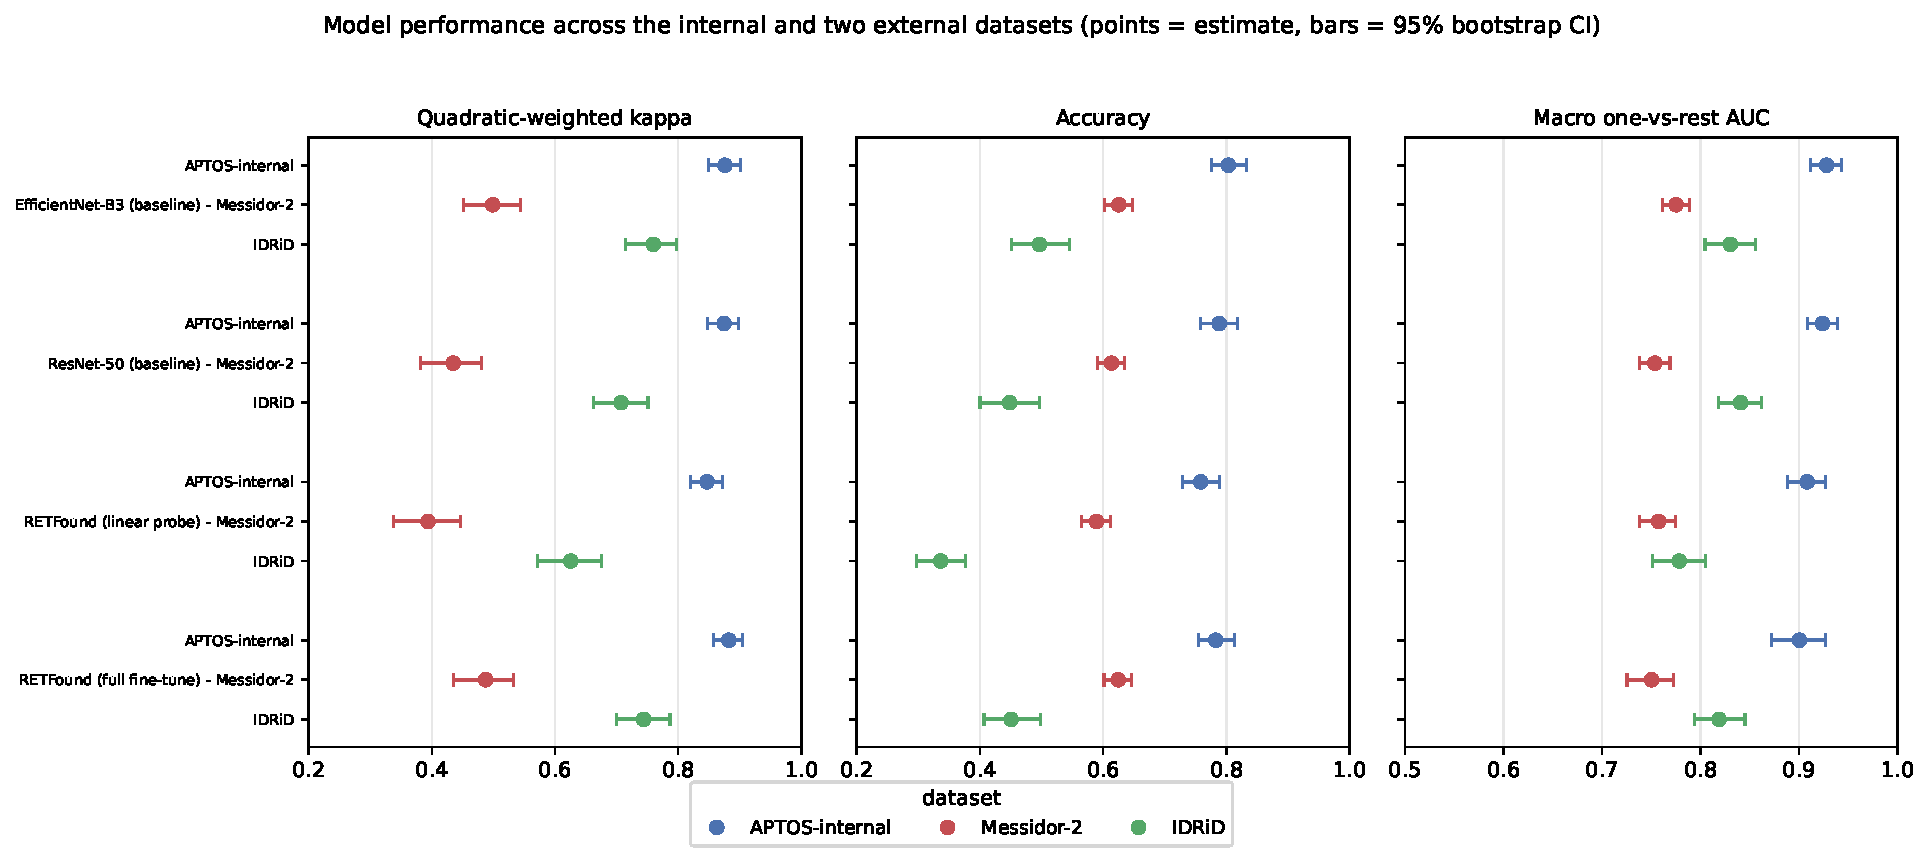
\includegraphics[width=\textwidth,height=0.44\textheight,keepaspectratio]{figures/fig_forest.pdf}
\caption{Model performance (quadratic-weighted kappa, accuracy, macro one-vs-rest
AUC) across the internal APTOS test set and the two external datasets. Points are
estimates; bars are $95\%$ bootstrap confidence intervals. The internal (blue)
versus external (red/green) gap is large and its confidence intervals do not
overlap for any model.}
\label{fig:forest}
\end{figure*}

\begin{figure*}[!t]
\centering
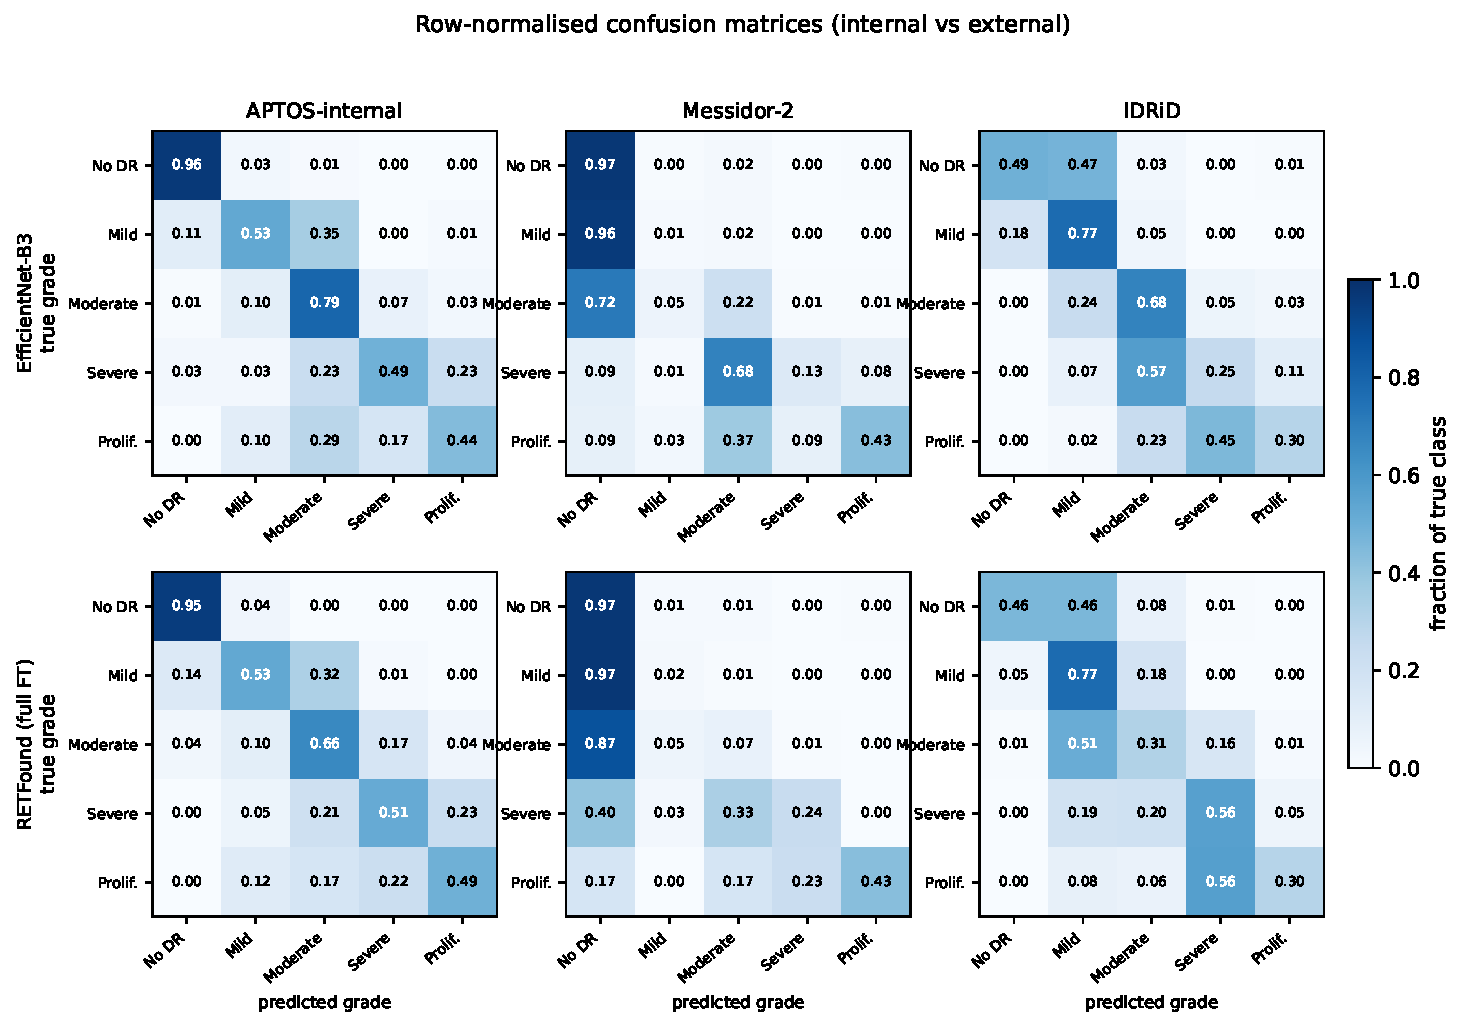
\includegraphics[width=\textwidth,height=0.46\textheight,keepaspectratio]{figures/fig_confusion.pdf}
\caption{Row-normalised confusion matrices for EfficientNet-B3 (top) and the
RETFound full fine-tune (bottom) on the internal APTOS test set and on the two
external datasets. On Messidor-2 both models collapse toward grade-0 and grade-2
prediction; on IDRiD the predictions shift toward more advanced grades, tracking
IDRiD's pathology-enriched class mix.}
\label{fig:confusion}
\end{figure*}

\begin{figure*}[!t]
\centering
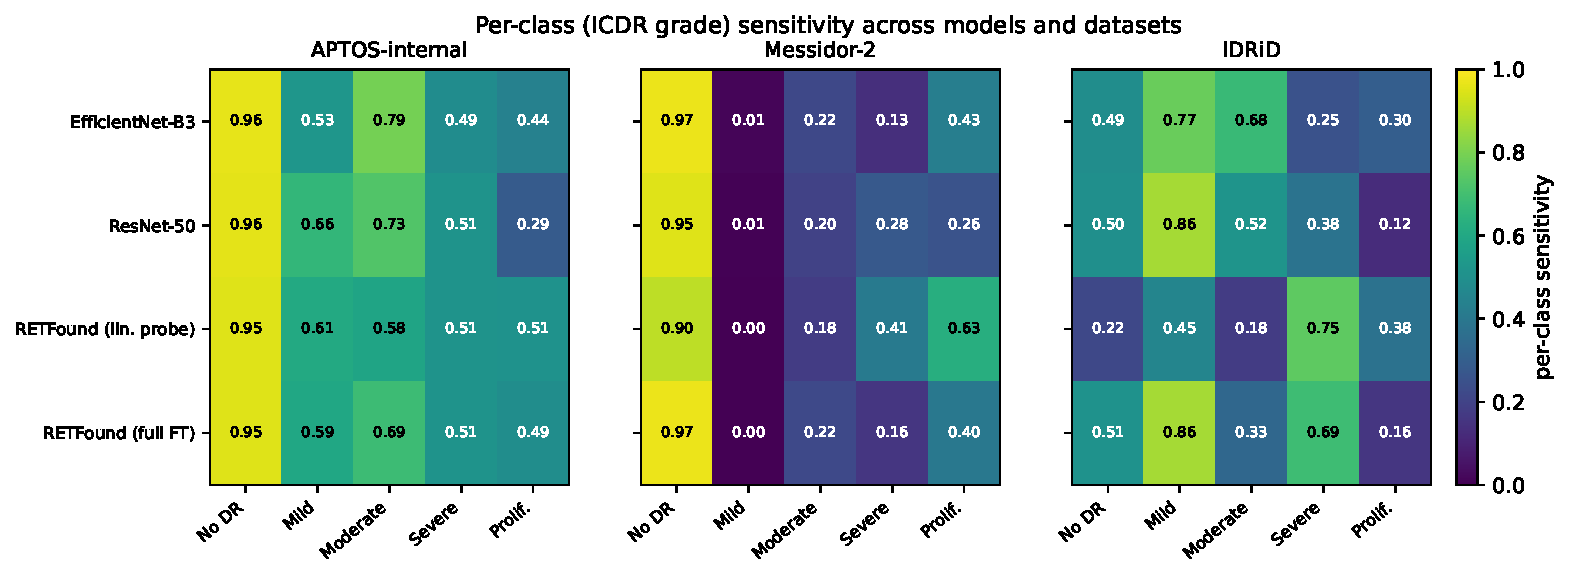
\includegraphics[width=\textwidth,height=0.34\textheight,keepaspectratio]{figures/fig_perclass.pdf}
\caption{Per-class (ICDR grade) sensitivity for every model on the internal and
two external datasets. On Messidor-2, grade-1 (mild) sensitivity is
$\leq 0.01$ for every model; RETFound retains isolated per-class advantages
(higher severe-grade sensitivity on IDRiD for both variants; highest
proliferative-grade sensitivity on Messidor-2 for the linear probe) without a
higher overall QWK.}
\label{fig:perclass}
\end{figure*}

Every model degraded on both external datasets (Tables~\ref{tab:master},
\ref{tab:drop}; Figures~\ref{fig:forest}, \ref{fig:confusion}). Degradation was
largest on Messidor-2, where QWK fell from $0.85$--$0.88$ internally to
$0.39$--$0.50$ and the $95\%$ CIs for the internal and external estimates did not
overlap for any model. On Messidor-2 all models reverted toward majority-class
(grade~0) prediction: grade-1 (mild) sensitivity was $\leq 0.01$ for every model
and grade-0 specificity fell to $0.26$--$0.32$ (Figure~\ref{fig:perclass}). On
IDRiD the QWK drop was smaller ($0.12$--$0.22$) but accuracy fell further
(drop $0.31$--$0.42$), consistent with IDRiD's pathology-enriched class mix
(Table~\ref{tab:datasets}, Figure~\ref{fig:grades}). Because the external
reference standards differ from APTOS's and from each other
(Section~\ref{sec:methods-refstd}), these absolute drops combine image shift with
a change of labelling protocol; the between-model contrasts below compare models
against the same labels.

\textbf{RQ1 --- Performance (primary outcome).} Fully fine-tuned RETFound did
not generalise better than the EfficientNet-B3 baseline, and it did not
generalise measurably worse. Its internal-to-external QWK drop exceeded the
baseline's by $+0.018$ on Messidor-2 ($95\%$ CI $[-0.024,0.058]$; Bonferroni
$98.75\%$ CI $[-0.036,0.068]$) and by $+0.022$ on IDRiD ($[-0.033,0.083]$;
$[-0.051,0.096]$), Holm-adjusted $p=0.79$ for both (Table~\ref{tab:drop}). Its
external QWK was close to the baseline's on both sets (paired difference
$-0.011$, $[-0.047,0.025]$ on Messidor-2; $-0.016$, $[-0.068,0.038]$ on IDRiD).
The confidence intervals exclude an advantage for RETFound larger than
$\approx 0.02$--$0.03$ QWK in drop, and also exclude a disadvantage larger than
$\approx 0.06$--$0.08$. The RETFound linear probe, in contrast, lost
significantly more ordinal agreement than the baseline on both external sets
($+0.076$, $[0.019,0.132]$, Holm $p=0.030$ on Messidor-2; $+0.105$,
$[0.038,0.170]$, Holm $p=0.016$ on IDRiD), and its external QWK was lower by
$0.105$ and $0.134$. So the pretrained RETFound representation, used frozen,
transferred worse than a fine-tuned ImageNet CNN, and full fine-tuning closed
that gap to parity but not beyond. ResNet-50, a secondary comparison, also lost
more than EfficientNet-B3 ($+0.063$ and $+0.051$; unadjusted).

For referable-DR discrimination (secondary; Table~\ref{tab:delong}; ROC and
precision--recall curves in Figure~\ref{fig:rocpr}), the baseline had a higher
AUC than the RETFound linear probe on both external sets (Messidor-2 $0.842$
vs.\ $0.781$; IDRiD $0.962$ vs.\ $0.903$; Holm $p<0.001$) and than the
full fine-tune on IDRiD ($0.962$ vs.\ $0.885$, Holm $p<0.001$). On Messidor-2
the full fine-tune's lower AUC ($0.817$, unadjusted $p=0.023$) did not survive
adjustment (Holm $p=0.11$), and no model differed from the baseline internally
(Holm $p\geq 0.31$). Per-class results (exploratory) show isolated RETFound
advantages under shift --- higher severe-grade (grade~3) sensitivity on IDRiD
for both variants ($0.69$--$0.75$ vs.\ $0.25$--$0.38$ for the CNNs) and, for the
linear probe, the highest proliferative-grade sensitivity and balanced accuracy
on Messidor-2 ($0.63$ and $0.42$) --- that reflect a different, not a more
accurate, error distribution (Figure~\ref{fig:perclassci};
\texttt{outputs/\allowbreak{}phase11/\allowbreak{}per\_class\_ci.csv}).

\textbf{Robustness of the primary inference.} (i) Treating every image as
having a perfectly correlated partner ($m=n/2$ bootstrap) widened every interval:
the full-fine-tune contrasts stayed null, the linear probe's IDRiD excess drop
still excluded zero ($[0.020,0.199]$), but its Messidor-2 interval reached zero
($[-0.004,0.157]$), as did both ResNet-50 intervals. Under the most pessimistic
dependence the linear probe's Messidor-2 deficit is therefore not
established, whereas its IDRiD deficit is. (ii) Re-weighting IDRiD to the
official grade mix changed IDRiD QWK by $\leq 0.015$ for every model and left
every IDRiD contrast unchanged (full fine-tune $+0.022$, $[-0.034,0.081]$; linear
probe $+0.117$, $[0.049,0.184]$). (iii) On the $T=20$ stochastic-pass
predictions (CNN head dropout and RETFound stochastic depth active; the linear
probe has no training-time stochastic layer and is therefore unchanged), the
full-fine-tune contrasts stayed null ($+0.019$, $[-0.024,0.062]$; $+0.035$,
$[-0.020,0.092]$; Holm $p=0.43$) and the linear-probe contrasts stayed
significant ($+0.071$, Holm $p=0.039$; $+0.105$, Holm $p=0.016$;
\texttt{outputs/\allowbreak{}phase23/\allowbreak{}*\_mc\_lpdet.*}). During
revision we found that the stochastic-pass script had rebuilt the linear probe's
frozen backbone with a drop-path rate of $0.2$ that it was never trained with;
those files are superseded and the script is corrected
(\texttt{outputs/\allowbreak{}phase8/\allowbreak{}mc\_lp\_deterministic/\allowbreak{}README.md}). The linear-probe
deficit is consistent in direction across all of these analyses, but under the
most pessimistic dependence assumption its Messidor-2 component is not
established; the full-fine-tune null is stable under all of them.

\subsection{Does the answer hold for referable DR? (secondary)}
\label{sec:results-referable}

To test whether the five-class result depends on the ordinal QWK metric, the
same internal-to-external drop analysis was repeated for the binary
referable-DR decision (ICDR grade $\geq 2$), on AUROC instead of QWK, with $95\%$
bootstrap CIs ($B=2000$; \texttt{scripts/\allowbreak{}phase19\_referable\_dr.py};
exploratory). On Messidor-2 the EfficientNet-B3 baseline's AUROC fell by $0.138$
($[0.115,0.161]$; internal $0.980\to$ external $0.842$), the RETFound full
fine-tune's by $0.150$ ($[0.122,0.180]$), and the other two models' by
$0.189$--$0.195$ (ResNet-50 $[0.162,0.215]$; linear probe $[0.169,0.223]$). On
IDRiD the baseline's AUROC barely moved ($0.018$, $[0.001,0.036]$), while both
RETFound variants lost more (linear probe $0.074$, $[0.045,0.103]$; full
fine-tune $0.082$, $[0.048,0.118]$). At each model's own operating point
(predicted grade $\geq 2$), referable sensitivity on Messidor-2 was low for every
model ($0.36$--$0.43$; full fine-tune $0.392$ vs.\ baseline $0.387$) at
specificity $0.90$--$0.98$, the same reversion to grade-0 prediction seen in the
five-class confusion matrices (Figure~\ref{fig:confusion}); on IDRiD the full
fine-tune's sensitivity was $0.760$ versus the baseline's $0.855$. The binary
task thus agrees with the five-class task on Messidor-2 (full fine-tune close to
the baseline, linear probe worse) and is less favourable to RETFound on IDRiD,
where the five-class parity of the full fine-tune does not carry over to
referable-DR ranking. Full operating-point metrics are in
\texttt{outputs/\allowbreak{}phase19/\allowbreak{}referable\_dr\_master.csv}.

\subsection{Can the models' uncertainty flag their errors? (RQ2)}
\label{sec:results-unc}

Every model lost substantial agreement externally, so the practical question is
whether a model knows when it is wrong.

\begin{figure*}[!t]
\centering
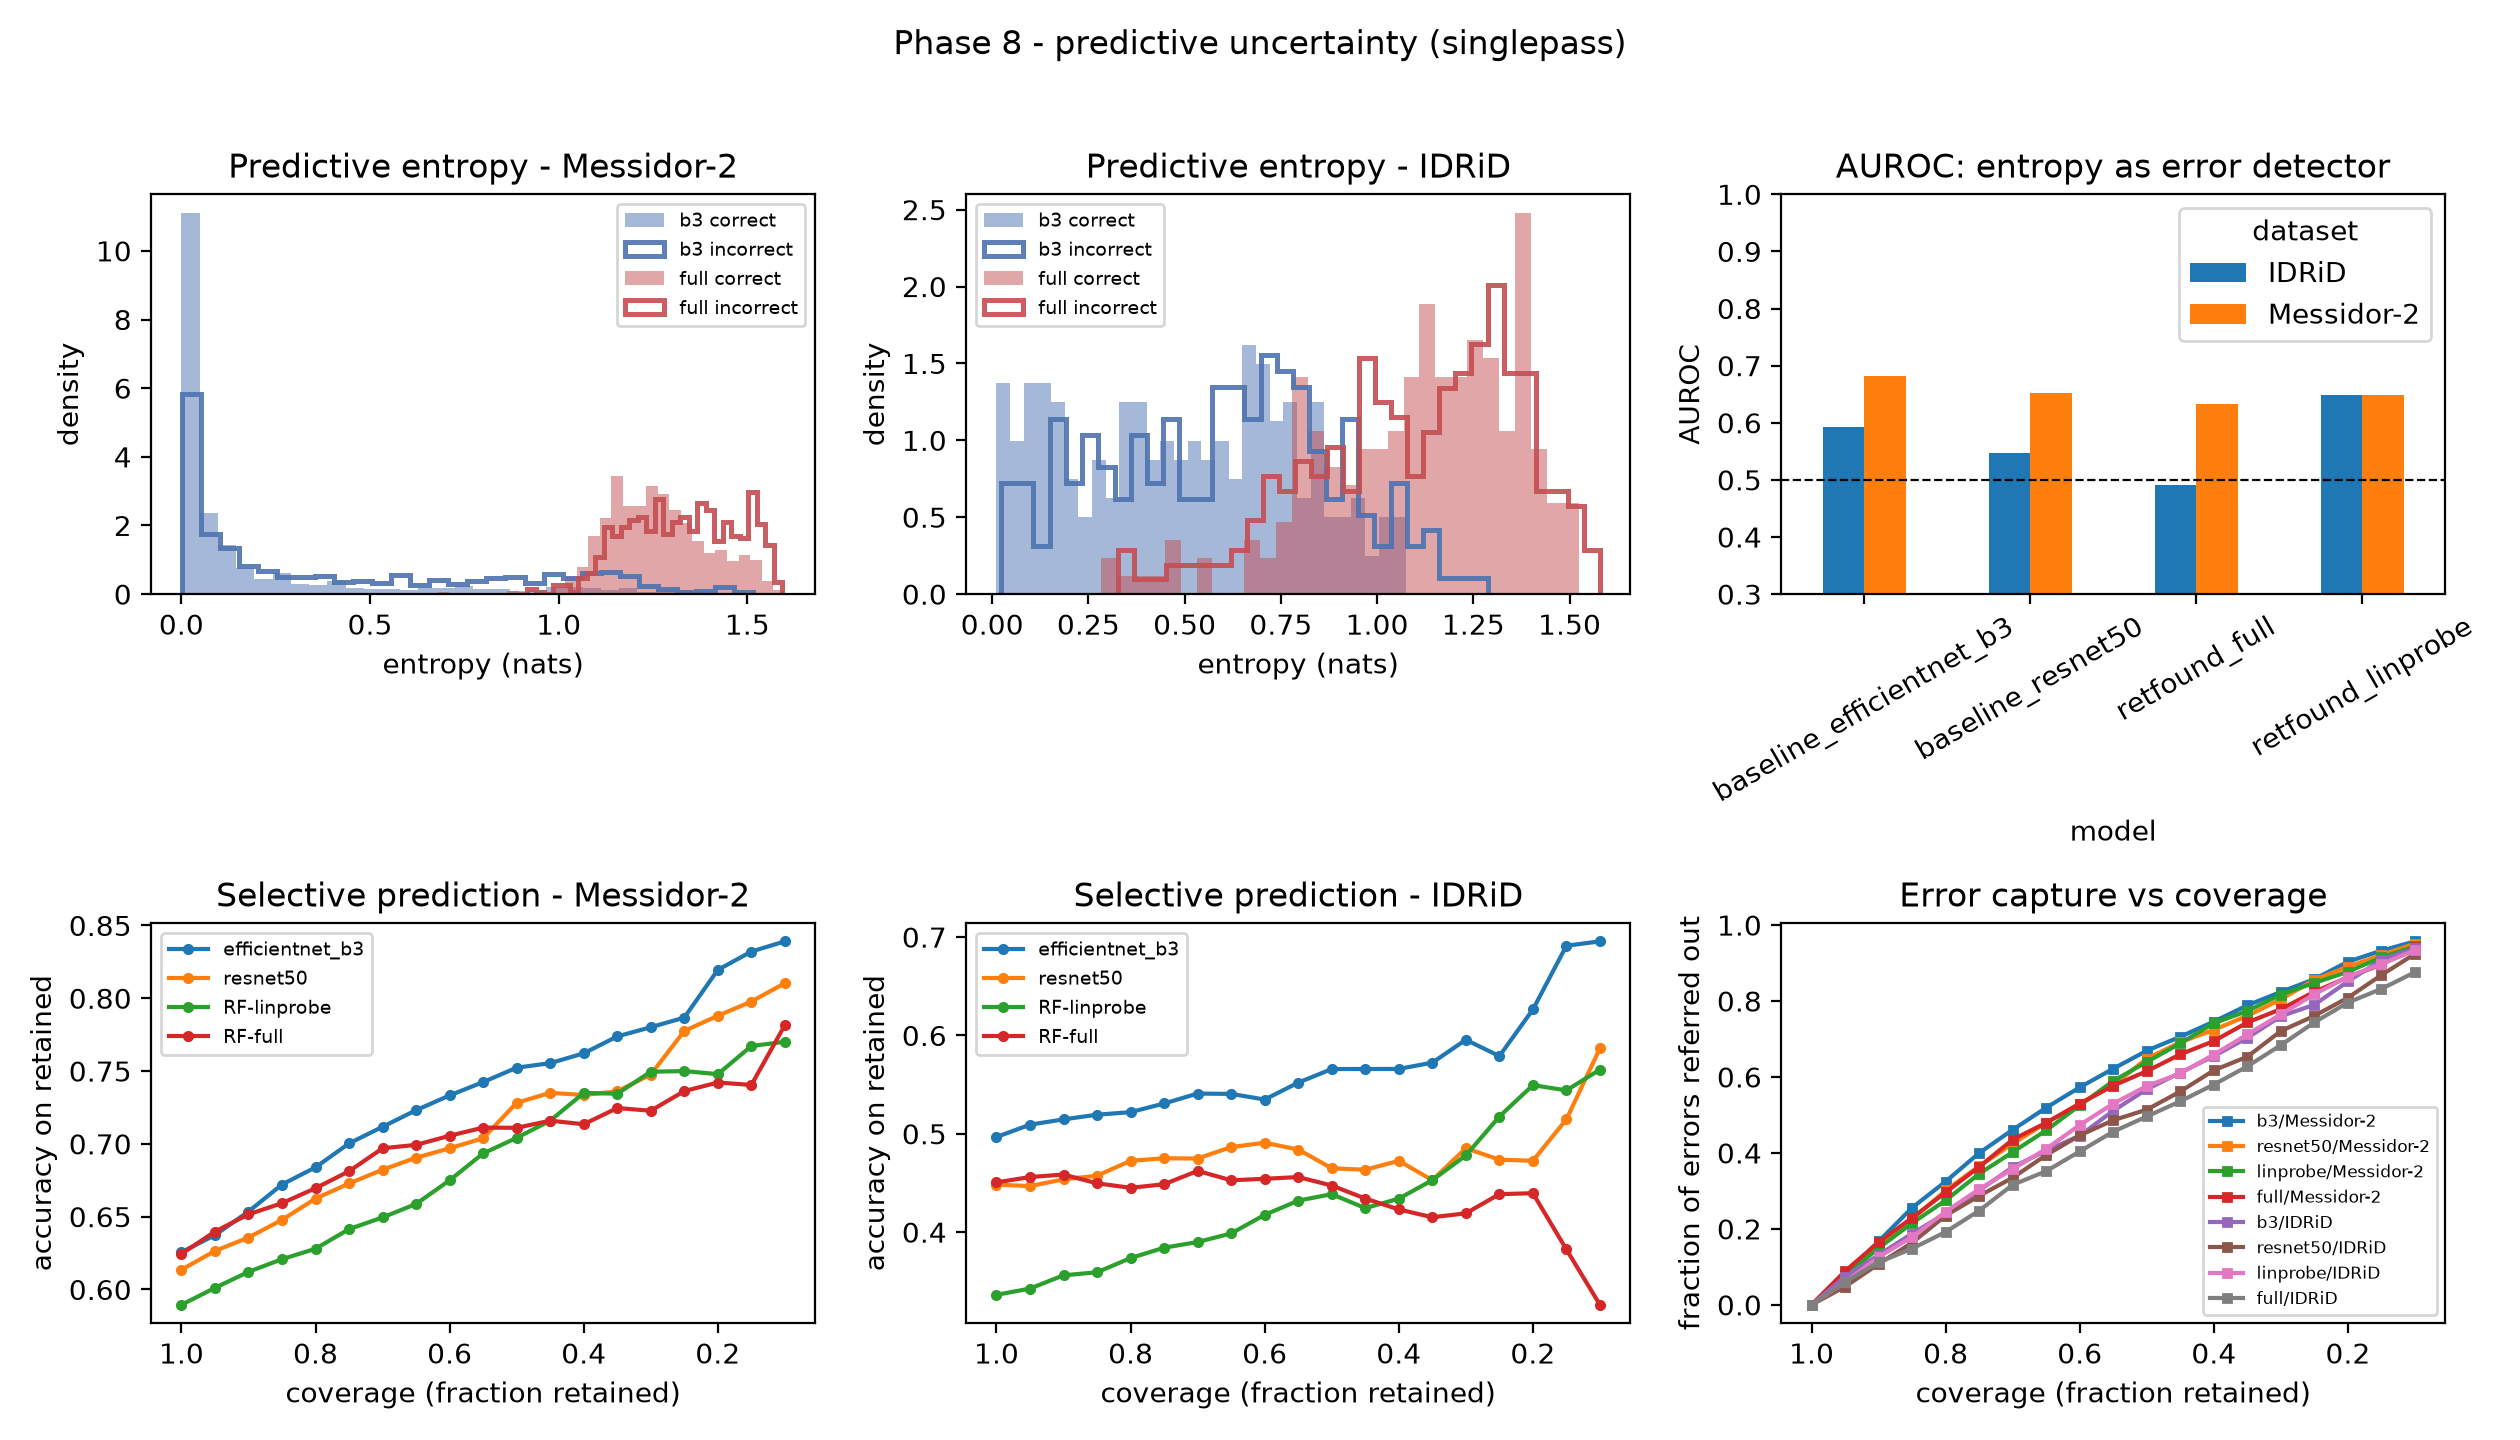
\includegraphics[width=\textwidth,height=0.48\textheight,keepaspectratio]{figures/fig_uncertainty.png}
\caption{Predictive uncertainty on external data. Top left/centre:
single-pass softmax-entropy distributions for correctly and incorrectly
classified images (EfficientNet-B3 and RETFound full fine-tune). Top right: AUROC of predictive
entropy as an error detector (dashed line, chance). Bottom: selective-prediction
curves (accuracy on retained cases, and fraction of all errors referred out,
versus retained coverage).}
\label{fig:uncertainty}
\end{figure*}

All results in this subsection use the primary measure, single-pass softmax
entropy, unless stated otherwise, and are exploratory. Internally, entropy
separated correct from incorrect predictions well for the CNNs (error-detection
AUROC: EfficientNet-B3 $0.84$, ResNet-50 $0.79$), moderately for the RETFound
linear probe ($0.69$), and not at all for the RETFound full fine-tune ($0.52$;
one-sided Mann--Whitney $p=0.26$). On external data the signal was weak for every
model (AUROC $0.49$--$0.68$; Figure~\ref{fig:uncertainty}). Misclassified images
carried significantly higher entropy than correct ones in most model $\times$
external-dataset cells ($p<0.001$), with two exceptions: ResNet-50 on IDRiD
($p=0.04$) and the RETFound full fine-tune on IDRiD, where entropy carried no
error signal (AUROC $0.49$, $p=0.63$). In selective-prediction terms, referring
the $10\%$ most uncertain external predictions captured only $11$--$17\%$ of the
errors on each external dataset, close to the $\approx 10\%$ expected from random
referral, versus $20$--$30\%$ internally. In the stochastic-pass sensitivity
analysis ($T=20$; CNNs and RETFound full fine-tune) every external
error-detection AUROC changed by $\leq 0.016$, the full fine-tune's internal AUROC
rose from $0.52$ to $0.56$, and its IDRiD AUROC stayed at chance ($0.49$,
$p=0.62$) (\texttt{outputs/\allowbreak{}phase8/\allowbreak{}uncertainty\_mc.csv}).

Breaking entropy down by ICDR grade
(\texttt{outputs/\allowbreak{}phase8/\allowbreak{}uncertainty\_by\_class\_singlepass.csv}) shows why the
foundation model's entropy is uninformative. For the CNNs, mean external entropy
tracked difficulty: EfficientNet-B3 on Messidor-2 rose from $0.15$ nats on
grade-0 images (where it was $97\%$ accurate) to $0.83$ nats on grade-3 images
($13\%$ accurate). The RETFound full fine-tune sat at $1.20$--$1.38$ nats across
every grade on Messidor-2 and $0.86$--$1.27$ on IDRiD, a large fraction of the
$\ln 5\approx 1.61$ maximum, whether its per-grade accuracy was $0.97$ or $0.00$;
the linear probe behaved the same way. Its entropy therefore reflects a
uniformly flat posterior rather than a data-dependent confidence, consistent with
label smoothing and the low fitted temperature (Section~\ref{sec:results-calib}).
The same holds by predicted grade: the $1527$ grade-0 predictions the full
fine-tune issued on Messidor-2 were wrong $35\%$ of the time yet carried
$1.28$-nat mean entropy, within the $1.12$--$1.55$ range of its other predicted
grades, so those errors were not flagged.

\subsection{Are the probabilities calibrated? (RQ2)}
\label{sec:results-calib}

Error detection depends on the ranking of confidence; calibration asks whether
the confidence values themselves can be taken at face value.

\begin{table*}[!t]
\centering\small
\caption{Calibration on the internal and external datasets: expected calibration
error (ECE, $15$ bins) with a $95\%$ bootstrap CI, maximum calibration error
(MCE), multi-class Brier score, and negative log-likelihood (NLL). Lower is
better throughout. Under external shift the ImageNet CNNs become markedly
over-confident (ECE $\approx 0.26$--$0.29$) while RETFound's flatter,
label-smoothed outputs stay closer to calibrated (ECE $\approx 0.09$--$0.13$).}
\label{tab:calib}
\setlength{\tabcolsep}{4pt}
\begin{tabular}{llcccc}
\toprule
Model & Dataset & ECE (95\% CI) & MCE & Brier & NLL \\
\midrule
\multirow{3}{*}{EfficientNet-B3}
 & APTOS-internal & 0.101 (0.080--0.129) & 0.295 & 0.300 & 0.645 \\
 & Messidor-2     & 0.279 (0.259--0.302) & 0.439 & 0.644 & 1.742 \\
 & IDRiD          & 0.294 (0.253--0.342) & 0.437 & 0.764 & 1.668 \\
\midrule
\multirow{3}{*}{ResNet-50}
 & APTOS-internal & 0.058 (0.046--0.091) & 0.308 & 0.311 & 0.608 \\
 & Messidor-2     & 0.265 (0.246--0.290) & 0.400 & 0.650 & 1.583 \\
 & IDRiD          & 0.260 (0.220--0.312) & 0.459 & 0.778 & 1.445 \\
\midrule
\multirow{3}{*}{RETFound (linear probe)}
 & APTOS-internal & 0.182 (0.159--0.211) & 0.250 & 0.395 & 0.815 \\
 & Messidor-2     & 0.121 (0.100--0.145) & 0.156 & 0.594 & 1.181 \\
 & IDRiD          & 0.127 (0.093--0.172) & 0.419 & 0.758 & 1.462 \\
\midrule
\multirow{3}{*}{RETFound (full fine-tune)}
 & APTOS-internal & 0.179 (0.161--0.213) & 0.258 & 0.370 & 0.748 \\
 & Messidor-2     & 0.095 (0.076--0.118) & 0.230 & 0.563 & 1.158 \\
 & IDRiD          & 0.129 (0.101--0.184) & 0.449 & 0.715 & 1.378 \\
\bottomrule
\end{tabular}
\end{table*}

\begin{figure*}[!t]
\centering
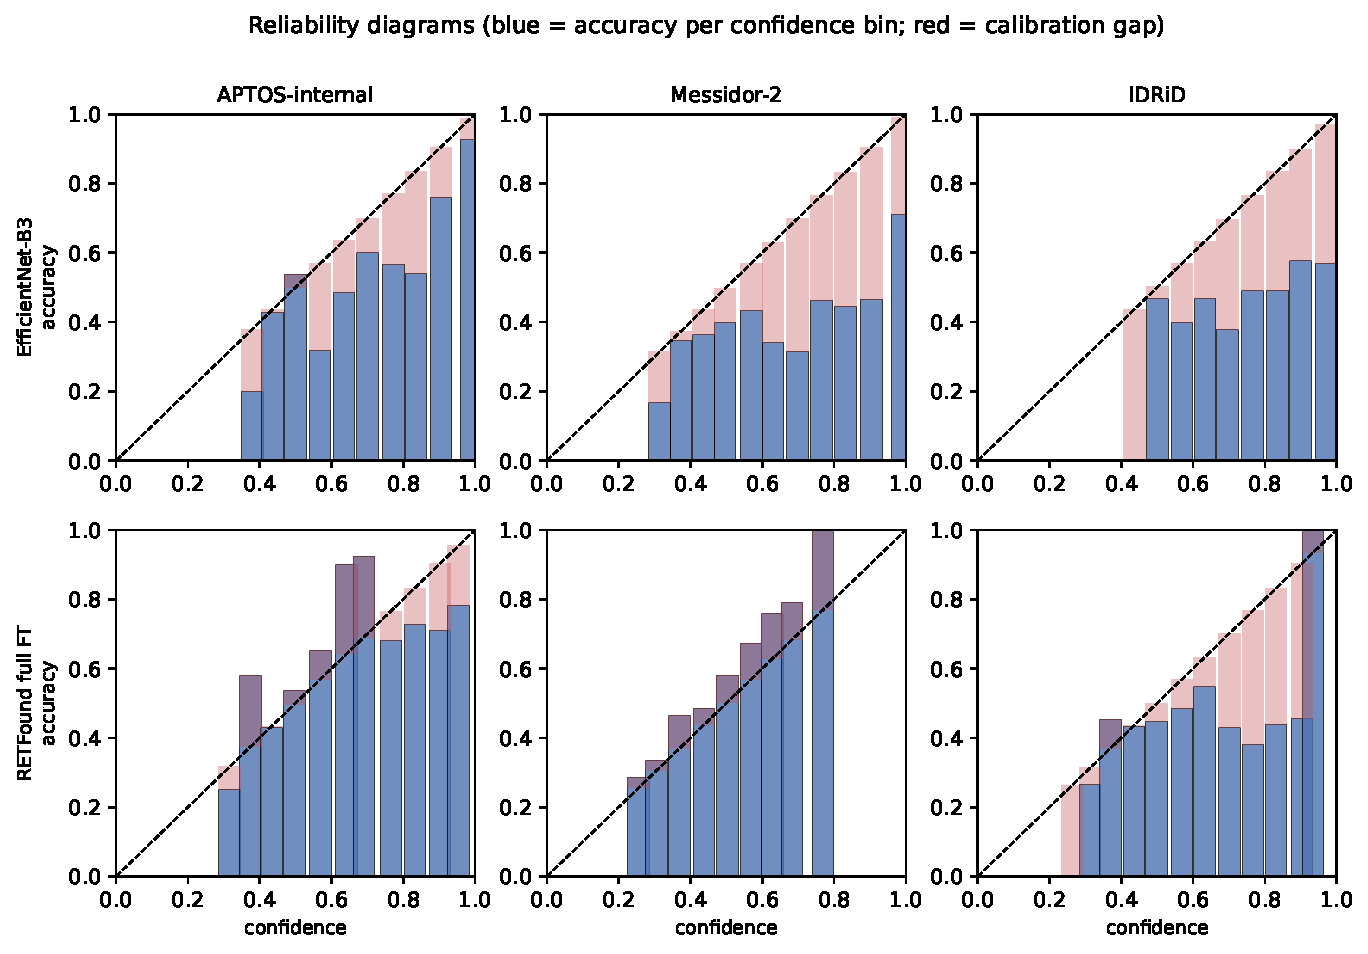
\includegraphics[width=\textwidth,height=0.42\textheight,keepaspectratio]{figures/fig_reliability.pdf}
\caption{Reliability diagrams for EfficientNet-B3 (top) and the RETFound full
fine-tune (bottom) on the internal test set and the two external datasets. Blue
bars are accuracy per confidence bin; red segments are the calibration gap.
Internally the CNN is close to the diagonal; externally it sits far below it
(over-confident). RETFound's diagram is flatter and closer to the diagonal on the
external sets.}
\label{fig:reliability}
\end{figure*}

Internally, the ImageNet CNNs were well calibrated (ECE $0.06$--$0.10$) and
RETFound less so (ECE $0.18$ for both variants; label smoothing $0.1$ during
fine-tuning flattens its softmax). Under external shift this reversed
(Table~\ref{tab:calib}, Figure~\ref{fig:reliability}; exploratory): both CNNs
became strongly over-confident (ECE $0.26$--$0.29$; Brier $0.64$--$0.78$),
whereas RETFound's ECE \emph{fell} to $0.09$--$0.13$ and its Brier score was
similar or lower ($0.56$--$0.76$). The foundation model's probability estimates
therefore degraded less under shift than its discrimination. This does not make
its external predictions reliable: a well-calibrated but near-uniform posterior
cannot separate its own errors (Section~\ref{sec:results-unc}).

\textbf{Recalibration.} Post-hoc temperature scaling did not repair external
miscalibration. Temperatures fitted on the APTOS validation split were $T>1$ for
the over-confident CNNs (EfficientNet-B3 $1.52$, bootstrap $95\%$ CI
$[1.32,1.71]$; ResNet-50 $1.16$, $[1.01,1.30]$) and $T<1$ for the
under-confident, label-smoothed RETFound variants (linear probe $0.50$,
$[0.43,0.58]$; full fine-tune $0.62$, $[0.54,0.70]$). Applied externally, the
fitted temperature lowered the CNNs' external ECE (EfficientNet-B3
$0.28\to0.21$ on Messidor-2, $0.29\to0.19$ on IDRiD) but left them clearly
over-confident, barely changed the RETFound full fine-tune on Messidor-2
($0.095\to0.090$), and \emph{worsened} both RETFound variants on IDRiD (full
fine-tune $0.13\to0.23$; linear probe $0.13\to0.30$), because IDRiD's shift runs
opposite in sign to Messidor-2's. Refitting $T$ on a disjoint stratified subset
of the APTOS \emph{training} split gave different temperatures (CNNs
$0.79$--$0.82$, RETFound $0.47$--$0.49$; the models are over-confident on images
they were trained on) and, applied externally, a higher ECE than no
recalibration in every external cell except the linear probe on Messidor-2
($0.121\to0.119$) (\texttt{outputs/\allowbreak{}phase13/\allowbreak{}traincalib/\allowbreak{}}). A recalibration constant learned
in-domain is therefore not a dependable external safeguard, and it is sensitive
to the choice of calibration data
(\texttt{outputs/\allowbreak{}phase13/\allowbreak{}temperature\_scaling.csv}).

\begin{figure*}[!t]
\centering
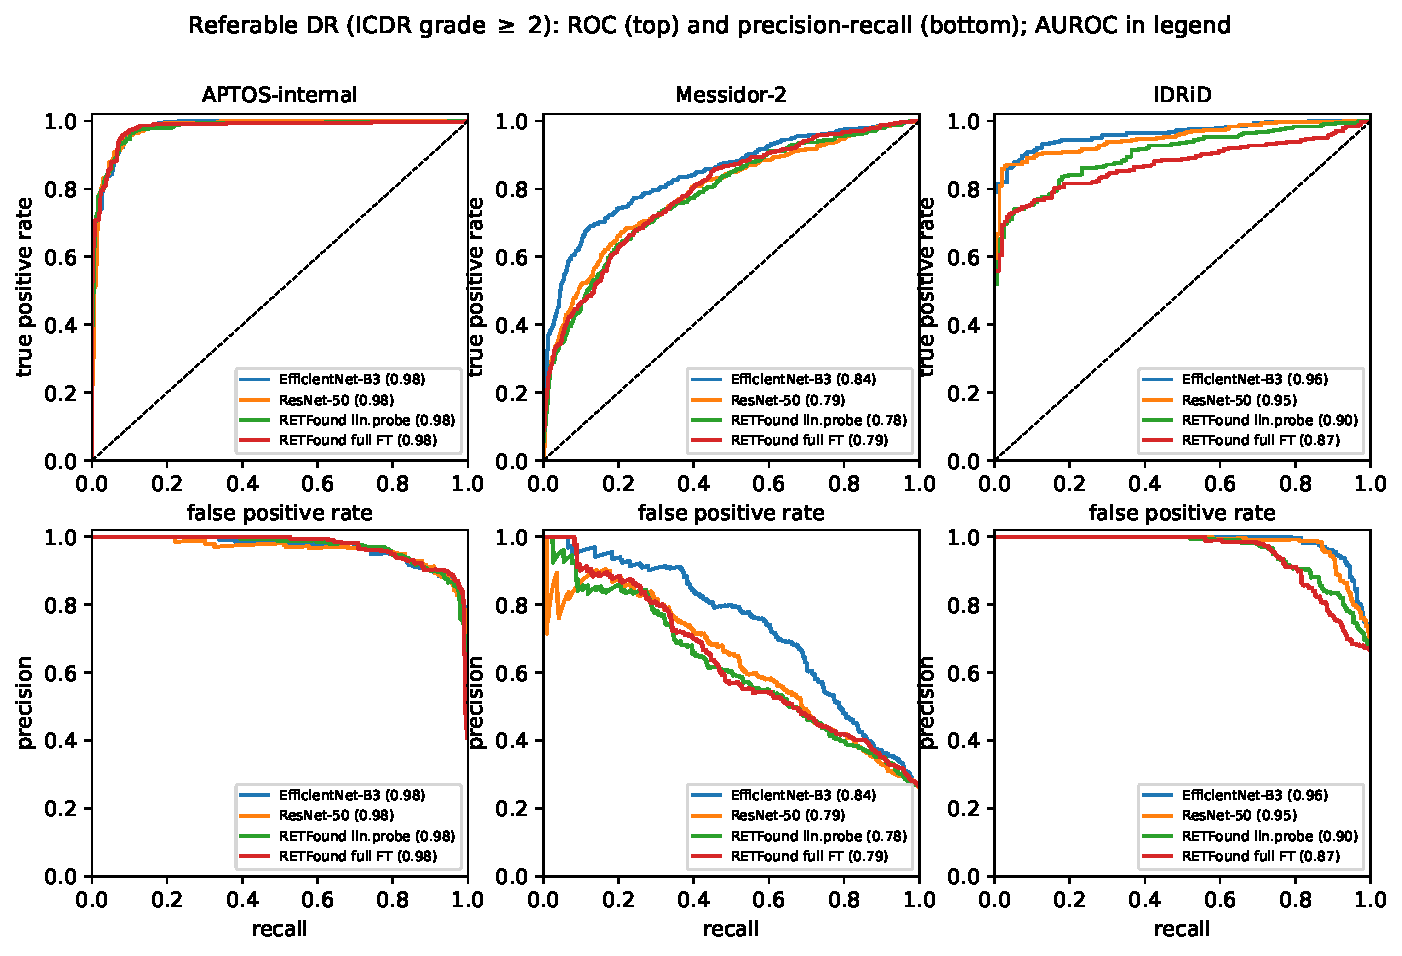
\includegraphics[width=\textwidth,height=0.44\textheight,keepaspectratio]{figures/fig_roc_pr.pdf}
\caption{Referable diabetic retinopathy (ICDR grade $\geq 2$): receiver operating
characteristic (top) and precision--recall (bottom) curves for every model on the
internal test set and the two external datasets; AUROC is in each legend. On both
external datasets the EfficientNet-B3 baseline has the highest AUC; the
differences are significant after adjustment for the linear probe on both sets
and for the full fine-tune on IDRiD (Table~\ref{tab:delong}).}
\label{fig:rocpr}
\end{figure*}

\begin{figure*}[!t]
\centering
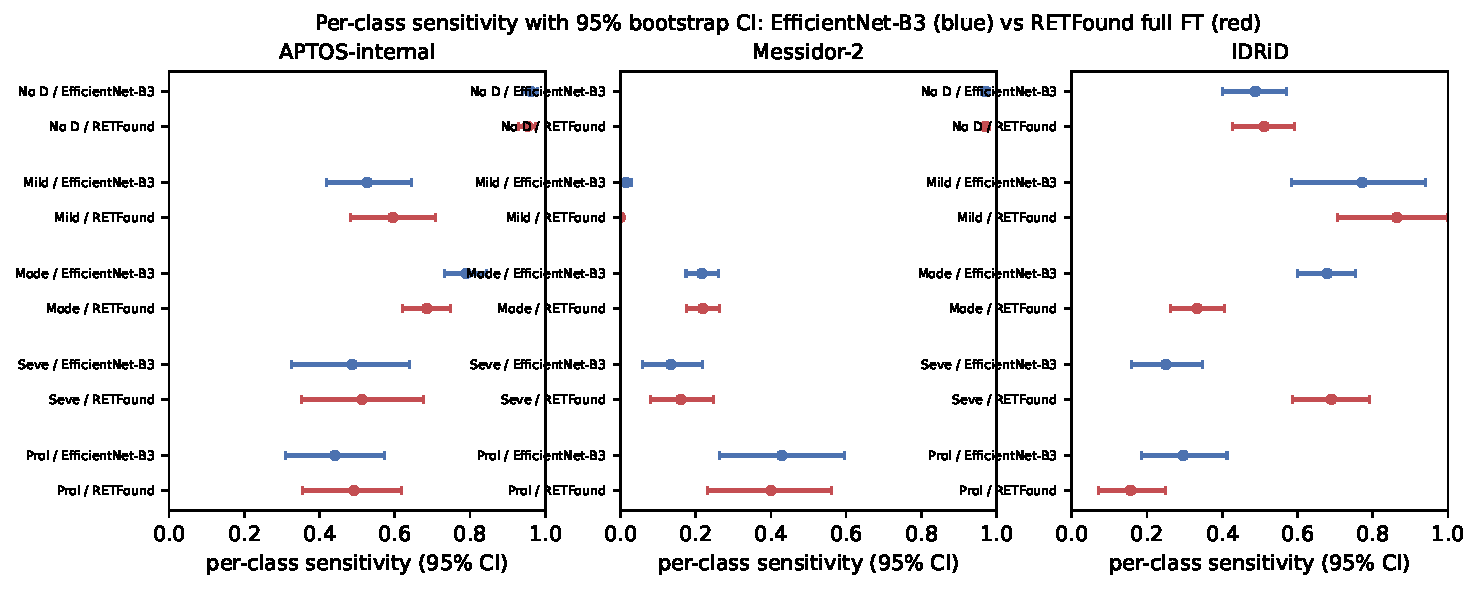
\includegraphics[width=0.85\textwidth,height=0.32\textheight,keepaspectratio]{figures/fig_perclass_ci.pdf}
\caption{Per-class sensitivity with $95\%$ bootstrap confidence intervals for
EfficientNet-B3 (blue) and the RETFound full fine-tune (red). Full per-class
sensitivity, specificity, precision, F1, and support with CIs for all four models
are in the supplement (\texttt{outputs/\allowbreak{}phase11/\allowbreak{}per\_class\_ci.csv}).}
\label{fig:perclassci}
\end{figure*}

\subsection{Can a generic shift detector do better? (RQ2)}
\label{sec:results-ood}

Because predictive entropy was a weak external error detector
(Section~\ref{sec:results-unc}), a domain-shift-specific alternative was tested:
a Mahalanobis distance-to-nearest-class-centroid score in a frozen, DR-naive
ImageNet EfficientNet-B3 feature space (class-conditional means and a
Ledoit--Wolf-shrunk shared covariance fit on APTOS-train only;
\texttt{scripts/\allowbreak{}phase20\_ood\_detection.py}), compared against each model's
own entropy as an error detector via a paired bootstrap on the AUROC
difference (exploratory). It did not help on the external sets. Across the
four models and two external datasets ($8$ cells) the Mahalanobis score was
never a significantly better error detector than entropy, and was significantly
\emph{worse} in $6$ of the $8$ (e.g.\ EfficientNet-B3 on Messidor-2: AUROC(OOD)
$0.472$ versus AUROC(entropy) $0.681$, difference $-0.210$, $95\%$ CI
$[-0.244,-0.176]$). The two remaining cells (ResNet-50 and the RETFound full
fine-tune, both on IDRiD) showed no significant difference; for the full
fine-tune this is because neither score carried a useful signal there
(AUROC $0.56$ and $0.49$). Internally, where the detector is fitted, the
pattern differed only for the RETFound full fine-tune: its entropy carried no
signal, so the generic distance score did better ($0.637$ vs.\ $0.516$, difference
$+0.121$, $[0.040,0.197]$), although still far below the CNNs' own entropy
($0.79$--$0.84$). A single generic, task-agnostic distributional-distance
score therefore does not substitute for a task-calibrated confidence signal on
these shifts; an out-of-distribution safeguard would need to be fitted or
validated on the deployment shift itself (per-cell results:
\texttt{outputs/\allowbreak{}phase20/\allowbreak{}ood\_master.csv}).

\subsection{Where do the models look? (RQ3, exploratory)}
\label{sec:results-explain}

The remaining analyses move from \emph{whether} the models fail to clues about
\emph{how}, and are exploratory.

\begin{figure*}[!t]
\centering
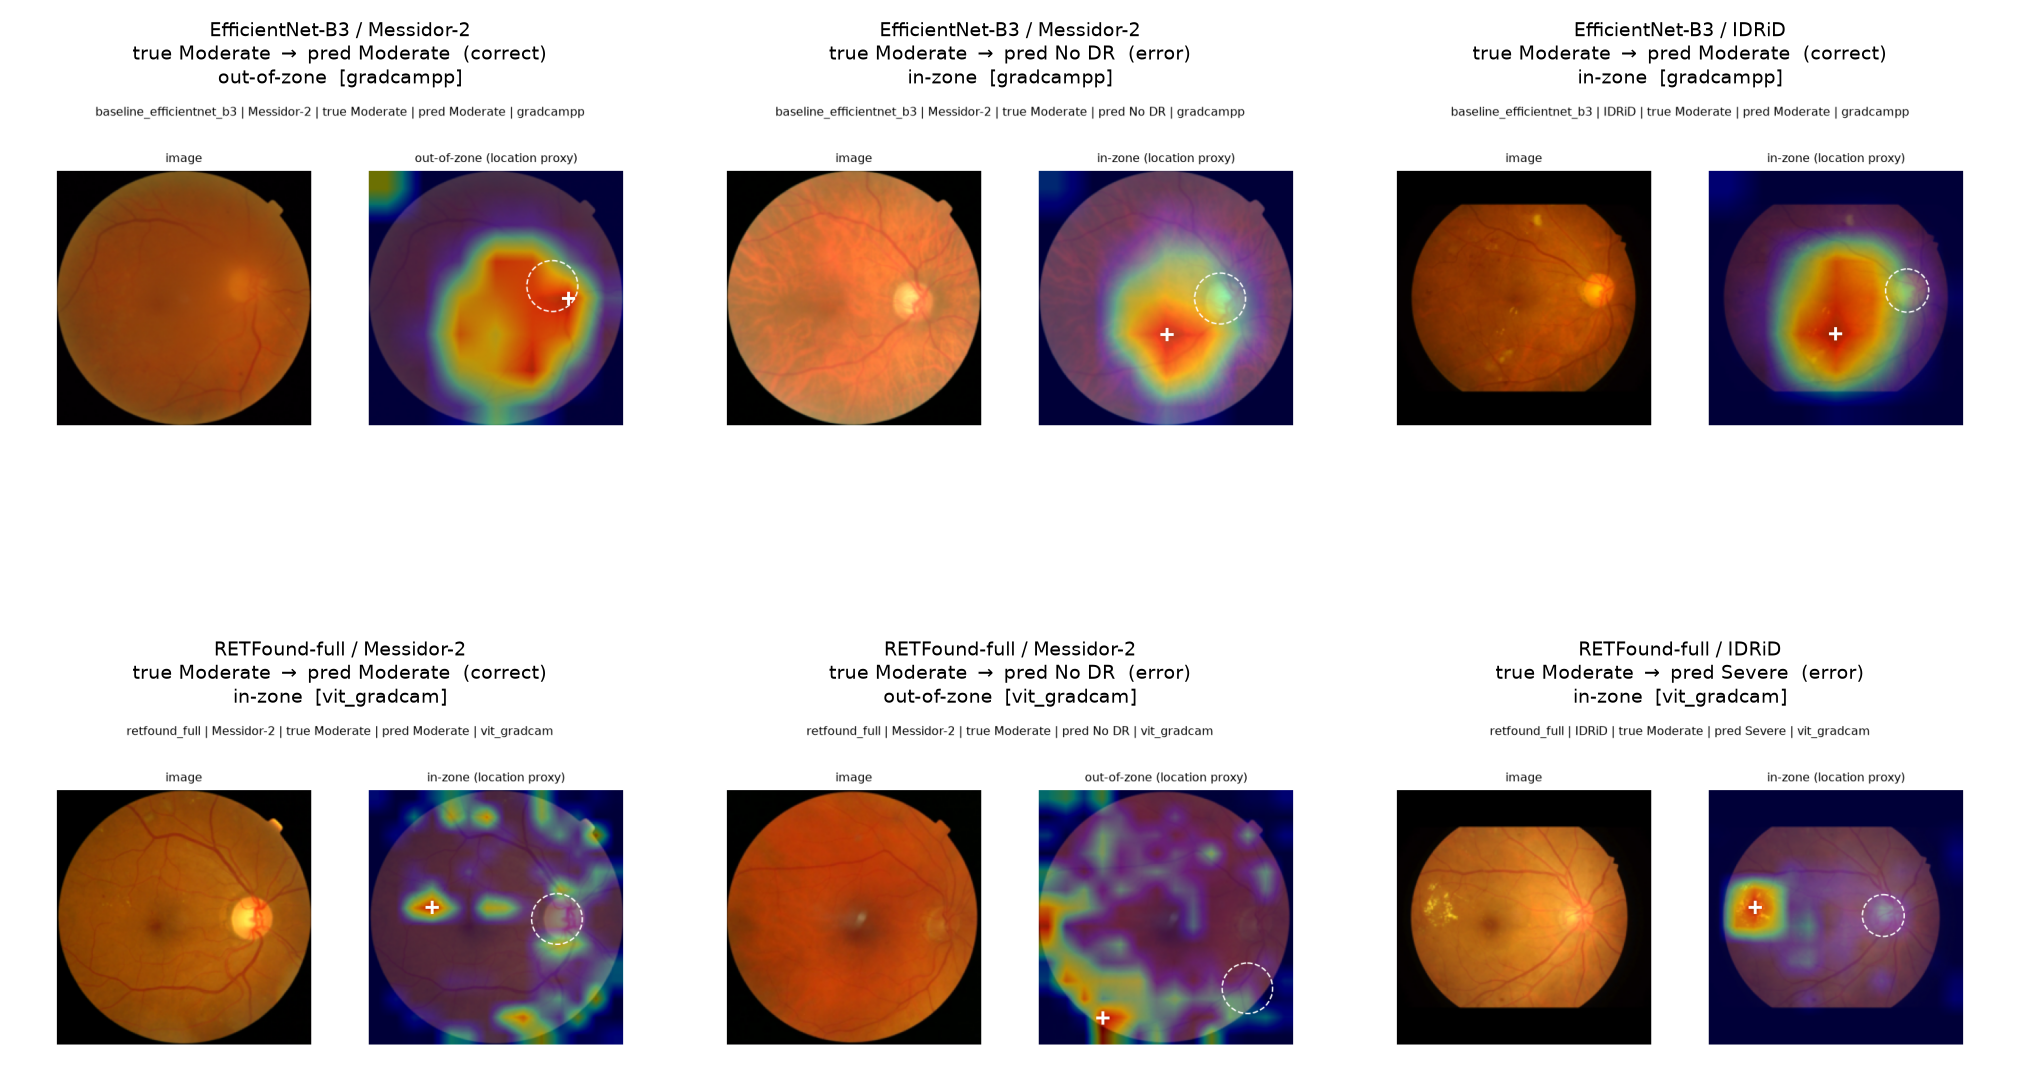
\includegraphics[width=\textwidth,height=0.42\textheight,keepaspectratio]{figures/fig_explainability.png}
\caption{Representative saliency maps on external images: EfficientNet-B3
(Grad-CAM++) and the RETFound full fine-tune (patch-token Grad-CAM), correctly
and incorrectly classified examples from Messidor-2 and IDRiD.
Dashed circle, estimated optic disc; white cross, saliency peak. Panel titles
give the true and predicted ICDR grade and the geometric location-proxy label
(in-zone / out-of-zone); this is not a lesion-level or expert assessment.}
\label{fig:explain}
\end{figure*}

Saliency maps were generated for a grade-stratified sample of external images
($40$ correctly and $25$ incorrectly classified per model per external dataset,
$65$ per cell). This analysis is exploratory and measures only \emph{where}
saliency falls (Section~\ref{sec:methods-explain}): an \emph{in-zone} map has its
peak and most of its top-decile mass inside the fundus and outside the estimated
optic-disc and border regions. It says nothing about whether the map is on a
lesion. The CNNs' Grad-CAM++ maps were in-zone for $90$--$100\%$ of maps in every
model $\times$ dataset $\times$ correctness cell, with $0.92$--$0.98$ of their
top-decile mass in the zone and $<4\%$ on the border annulus. RETFound's
patch-token Grad-CAM maps were in-zone less often: on IDRiD $83\%$ (full
fine-tune) and $72\%$ (linear probe), and on Messidor-2 $63\%$ and $46\%$, versus
$94\%$ for both CNNs. On Messidor-2 the difference came from saliency mass on
the outer border annulus: $17\%$ of the top-decile mass for the full
fine-tune's correct predictions and $29\%$ for its errors ($29\%$ and $50\%$ for
the linear probe). Figure~\ref{fig:explain} shows representative panels;
per-cell rates are in \texttt{outputs/\allowbreak{}phase7/\allowbreak{}plausibility\_rates.csv}.
Two caveats limit interpretation. First, an in-zone map is not evidence of
lesion focus: the zone also contains vessels, the macula, and normal retina,
and we did not test overlap with lesions. Second, ViT patch-token Grad-CAM and
CNN Grad-CAM++ differ in resolution and in how they distribute mass, so part of
the border difference may reflect the attribution method rather than the
model. The finding that can be stated is narrow: on Messidor-2, a larger share of
RETFound's attribution mass lay on the image border, more so for its errors. A
blinded rating packet and scorer for a two-rater expert assessment are released
(Section~\ref{sec:methods-explain}) but have not been completed.

\subsection{How sensitive are the models to the input distribution? (exploratory)}
\label{sec:results-ablation}

To probe how sensitive each model is to the input distribution (exploratory),
external inference was re-run (no retraining) for EfficientNet-B3 and the RETFound
full fine-tune under two inference-time input perturbations: CLAHE contrast
equalisation, and a colour-transfer that maps each image's fundus-pixel channel
statistics to the APTOS training distribution
(\texttt{scripts/\allowbreak{}phase15\_ablation.py}). Neither improved RETFound's
external ordinal agreement; both reduced it, and the foundation model was far more
fragile than the CNN. The colour-transfer left EfficientNet-B3 close to
unchanged on Messidor-2 (QWK $0.499\to0.512$) and lowered it on IDRiD
($0.760\to0.689$), but pushed the RETFound full fine-tune down on every set,
including the internal one (APTOS-internal $0.882\to0.811$, Messidor-2
$0.487\to0.284$, IDRiD $0.744\to0.693$). CLAHE was worse still for RETFound
(APTOS-internal $0.882\to0.703$, Messidor-2 $0.487\to0.096$, IDRiD
$0.744\to0.410$) while affecting the CNN much less ($0.876\to0.807$ internal,
$0.499\to0.458$ on Messidor-2, $0.760\to0.697$ on IDRiD). Because the
perturbations are applied at inference to models trained on unperturbed images,
this measures sensitivity to an input-distribution shift, not the value of
training with these normalisations. It shows that the fully fine-tuned ViT's
predictions are tightly coupled to the APTOS colour and contrast distribution,
whereas the CNN absorbs the same perturbations.

A third variant tested input resolution: all three test sets were
re-preprocessed from their source images at $384$~px and both models were re-run
without retraining, the RETFound ViT-L built at $384$~px with its $224$-trained
positional embedding bicubically interpolated onto the $24{\times}24$ token grid
(\texttt{scripts/\allowbreak{}phase15c\_resolution.py}). The two models responded in
opposite directions on the two external sets. RETFound's Messidor-2 QWK rose
($0.487\to0.553$) while its IDRiD QWK fell ($0.744\to0.652$), with internal QWK
unchanged ($0.882\to0.886$), confirming the interpolation is benign in-domain.
EfficientNet-B3, trained at $224$, lost internal QWK at $384$
($0.876\to0.824$) and lost external QWK on both sets (Messidor-2
$0.499\to0.425$, IDRiD $0.760\to0.731$). The change in internal-to-external drop
from switching to $384$~px was $-0.062$ / $+0.096$ for RETFound and $+0.022$ /
$-0.024$ for EfficientNet-B3 (Messidor-2 / IDRiD;
\texttt{outputs/\allowbreak{}phase15c/\allowbreak{}}). Working resolution therefore
interacts with the shift in a dataset-specific way, and at $384$~px RETFound would
have outscored the CNN on Messidor-2 and underscored it on IDRiD; we report the
pre-specified $224$~px analysis as primary and make no claim that either model is
favoured by resolution in general. A colour- and
resolution-normalised \emph{retraining} comparison remains the definitive test
of the mechanism and is distinct from the inference-time perturbations above,
which show sensitivity to a shift applied to an already-trained model, not
whether training under that same transform would change what the model learns.
The data preparation and \texttt{train\_baseline.py} /
\texttt{train\_retfound.py --manifest ... --img-size ...} support for this
retraining comparison, and for a training-set-size sweep, are now released
(\texttt{scripts/\allowbreak{}phase18\_retrain\_variants\_prep.py},
\texttt{scripts/\allowbreak{}phase21\_training\_size\_sensitivity.py},
\texttt{COLAB\_RETRAIN\_GUIDE.md}); execution needs sustained GPU time beyond
this study's single consumer GPU (Section~\ref{sec:limitations}) and remains
outstanding.


\subsection{Is the linear-probe deficit a head artefact?}
\label{sec:results-headsummary}

A single linear layer might be too weak a head for frozen ViT features, which
would make the linear-probe deficit an artefact of our design rather than a
property of the representation. We tested this directly (exploratory; full
design and tables in Appendix~\ref{sec:results-headdepth}). On frozen features of
both backbones, $210$ heads were fitted ($0$ or $3$--$7$ hidden layers $\times$ four
activations $\times$ five seeds) and each scored unchanged on all three test sets.
Head depth moved internal QWK no more than reseeding did for either backbone, and
on Messidor-2 every one of the $21$ EfficientNet-B3 head configurations
(lowest cell mean $0.496$) outscored every one of the $21$ frozen-RETFound
configurations (highest $0.448$). The heads that internal validation would
favour for RETFound (deep GELU heads) were among the worst on Messidor-2. On
IDRiD the picture is less clear-cut: with both linear heads re-fitted under one
protocol the two backbones nearly tied ($0.720$ vs.\ $0.716$). The linear probe's
Messidor-2 deficit is therefore not a head artefact; its IDRiD deficit depends
partly on how the head is trained.

\section{Discussion}
\label{sec:discussion}

The study set out to test a widely held expectation: that a retinal foundation
model, having learned from many retinas rather than from everyday objects,
would hold up better than an ImageNet CNN when moved to a new dataset. Under a
matched protocol it did not, and it did not do worse either; used without
fine-tuning, it did worse. All models degraded, and none could tell when it was
wrong. We take the questions in turn.

\textbf{RQ1 --- Performance.} Under a matched preprocessing, fine-tuning, and
evaluation protocol, fully fine-tuning RETFound on APTOS~2019 did not yield
better cross-dataset generalisation for five-class DR grading than an
ImageNet-pretrained CNN. It did not yield measurably worse generalisation
either: its excess internal-to-external QWK drop over EfficientNet-B3 was
$+0.018$ on Messidor-2 and $+0.022$ on IDRiD, with intervals that include zero
and exclude an advantage for RETFound larger than about $0.02$--$0.03$. The
linear-probe variant generalised significantly worse than the CNN on both
external sets after family-wise correction. So retinal-domain pretraining,
used as a frozen representation, transferred \emph{less} robustly than a
fine-tuned ImageNet CNN, and adapting the whole network to APTOS brought it to
parity but not beyond. This does not contradict RETFound's reported strengths on
other tasks and modalities, but it tempers the expectation that retinal-domain
self-supervised pretraining confers robustness to the specific shifts
represented by Messidor-2 and IDRiD. Two qualifications apply. First, on IDRiD
the five-class parity did not carry over to the referable-DR decision, where the
full fine-tune ranked images less well than the CNN (AUC $0.885$ vs.\ $0.962$);
the IDRiD copy is incomplete and partly relabelled
(Section~\ref{sec:methods-idrid}), so this secondary finding needs confirmation on
the official release. Second, the full fine-tune is a single training run (seed
$42$); its contrast with the CNN ($+0.018$ on Messidor-2) is smaller than the
CNN's own seed-to-seed standard deviation of the Messidor-2 drop ($0.025$;
Section~\ref{sec:limitations}), which is consistent with parity but means a
small difference in either direction cannot be excluded.

\textbf{What changed from the interrupted run.} An earlier analysis of this study
used a RETFound full fine-tune stopped at epoch~$6$ by hardware limits and
reported that it generalised significantly worse than the CNN on Messidor-2
($\Delta$drop $+0.124$, $95\%$ CI $[0.074,0.175]$). Running the pre-specified
protocol to completion (best validation epoch $21$ of $28$) raised external QWK
from $0.368$ to $0.487$ on Messidor-2 and from $0.720$ to $0.744$ on IDRiD,
although validation QWK changed only from $0.935$ to $0.939$. Two lessons
follow: internal validation QWK did not predict external behaviour, and an
early-stopped checkpoint can misrepresent a model's generalisation by a margin
larger than any between-model difference in this study. The superseded results
are retained (\texttt{outputs/\allowbreak{}\_archive\_provisional\_epoch6/}).

\textbf{Nature of the shift.} The Messidor-2 collapse is an ordinal-structure
failure: models predict almost exclusively grade~0 or grade~2
(Figure~\ref{fig:confusion}), so accuracy is partly preserved by the high grade-0
prevalence while QWK falls sharply. The IDRiD pattern is different --- a base-rate
shift toward more advanced disease --- so accuracy falls more than QWK. Part of
both drops reflects a change of reference standard rather than of images:
Messidor-2 labels are an adjudicated three-specialist consensus, APTOS labels a
single clinician's, and IDRiD's grading process is not fully reported
(Section~\ref{sec:methods-refstd}). The absolute drops should therefore not be
read as pure measures of image-domain shift, and QWK should not be compared
across the two external sets; the between-model contrasts, which hold labels
fixed, are the robust part of the result.

\textbf{RQ2 --- Uncertainty and calibration.} Single-pass softmax entropy was at best a weak
error signal under dataset shift. It separated correct from incorrect predictions
internally for the CNNs (AUROC up to $0.84$), only weakly externally
($0.49$--$0.68$), and for the RETFound full fine-tune not even internally
($0.52$). Referring the most uncertain $10\%$ of external predictions would
capture $11$--$17\%$ of errors, barely better than referring a random $10\%$. A
generic out-of-distribution score was no better externally
(Section~\ref{sec:results-ood}). Neither the models' own confidence nor a generic
distributional-distance signal reliably flags external errors here; a safeguard
would have to be fitted and validated on the target domain. Calibration told a
partly different story: RETFound's label-smoothed probabilities were better
calibrated externally than the CNNs' (ECE $0.09$--$0.13$ vs.\ $0.26$--$0.29$),
but a well-calibrated, near-uniform posterior still cannot rank its own errors,
and temperatures fitted in-domain did not transfer
(Section~\ref{sec:results-calib}). Good calibration and useful uncertainty are
different properties, and only the first held for RETFound.

\textbf{RQ3 --- Explainability (exploratory).} The planned question --- whether
saliency overlaps DR lesions --- could not be answered, because neither lesion
masks nor blinded expert raters were available. What was measured is narrower: a
geometric location proxy showed RETFound's patch-token Grad-CAM placing more
attribution mass on the outer image border on Messidor-2 than the CNN's
Grad-CAM++ did ($17$--$29\%$ vs.\ $<4\%$ for the full fine-tune and the CNNs),
more so for its errors. This is compatible with, but does not demonstrate,
reliance on acquisition cues at the image edge, and part of it may reflect the
different attribution methods. We make no claim that either model's saliency is
lesion-focused or clinically plausible.

\textbf{Comparison with the literature.} Our finding agrees in direction with
the closest prior work. Hou et al.\ \cite{hou2025dinov2}, using the same three
public datasets, found that the retina-specific RETFound did not outperform a
natural-image foundation model for DR detection; we find that it also did not
outperform a supervised ImageNet CNN once both were trained identically. The two
studies differ in comparator, metric (AUC there, the drop in QWK here), and
protocol, so they corroborate rather than replicate each other. External
validation of DR systems more often reports referable-DR sensitivity and
specificity than five-class QWK, and QWK drops of the size seen here
($0.38$--$0.45$ on Messidor-2) are seldom reported, partly because five-class
external validation against an adjudicated reference standard is uncommon
\cite{grzybowski2020review}. Where cross-population degradation of DR models has
been quantified it is substantial \cite{dai2021spectrum,beede2020}; our results add
that, under a matched protocol, a retinal foundation model degraded as much as an
ImageNet CNN rather than less.

\textbf{Mechanism (speculative).} The retraining-based ablations that would test
mechanisms are prepared but not executed (Section~\ref{sec:limitations}), so the
following is interpretation. Three observations suggest that the fully
fine-tuned ViT is tightly coupled to APTOS acquisition statistics: it was far
more fragile than the CNN to inference-time colour and contrast perturbations,
internal set included (Section~\ref{sec:results-ablation}); its saliency placed
more mass on the image border on Messidor-2 (Section~\ref{sec:results-explain});
and its external performance moved substantially with input resolution, in
opposite directions on the two external sets. That this coupling coexists with
external QWK equal to the CNN's suggests that the two model families fail
differently rather than that one is more robust; an APTOS-only versus
multi-dataset training comparison and a normalised retraining ablation are the
direct tests.

\textbf{Implications.} These are retrospective experiments on public datasets,
and no result here supports using any of these models to screen patients or to
inform clinical decisions. Every model's five-class agreement fell from
$\approx 0.85$--$0.88$ internally to $0.39$--$0.50$ on Messidor-2, with grade-1
sensitivity $\leq 0.01$ and referable-DR sensitivity of $0.36$--$0.43$ at the
models' own operating points, and uncertainty did not flag the errors. The
methodological implication is that internal performance near QWK $0.9$, and the
use of a domain-specific foundation model, gave no assurance about behaviour on
images from a new camera, population, or grading protocol. Claims of robustness
for retinal AI should rest on external validation against an independent,
ideally adjudicated, reference standard, and any clinical use would require
prospective evaluation in the intended setting.


\section{Limitations}
\label{sec:limitations}

\textbf{Internal validity.} The RETFound full fine-tune ran the pre-specified
protocol to completion (early stopping on APTOS validation QWK at epoch $28$,
best epoch $21$; \texttt{CHECKPOINTS.md}), but as a single run; the
CNN baseline and the linear probe have four seeds each, the full fine-tune
one, because each run takes several hours on the single consumer GPU used. All
numbers come from one codebase on one machine with no independent
re-implementation, mitigated by releasing the code, checkpoint hashes, the exact
environment, and per-image predictions (Section~\ref{sec:repro}). The internal
APTOS split is image-level, not patient-level, because APTOS has no patient
identifiers; fellow-eye or repeat images may span the split and make internal
estimates optimistic. Byte-identical duplicates ($41/733$ internal-test images)
were checked and change internal QWK by $\leq 0.006$
(Section~\ref{sec:methods-split}).

\textbf{External validity.} All datasets are retrospective and public, and no
prospective or clinical claim is made. The IDRiD copy contains $455$ of the
official $516$ images, under-represents grade~0, and has at least $7$ labels that
differ from the official grades (Section~\ref{sec:methods-idrid}); grade
re-weighting changed no conclusion, but the label discrepancy is not corrected,
and all IDRiD results should be confirmed on the official release. The three
reference standards were produced by different processes
(Section~\ref{sec:methods-refstd}), so absolute drops conflate image shift with
labelling protocol and QWK is not comparable across the external sets. External
sample sizes limit precision for rare grades --- grade-1 sensitivity is
effectively not estimable on Messidor-2. One retinal foundation model and one
downstream task were studied, and the result should not be generalised to other
foundation models or tasks without direct testing.

\textbf{Construct validity.} Saliency was assessed only by a geometric location
proxy; no lesion masks or blinded expert grading were used, the proxy cannot
distinguish lesion, vessel, or normal-retina activation within the fundus zone,
and the CNN and ViT attribution methods differ. RQ3 is therefore unanswered as
originally posed. The blinded rating packet, rubric, and scorer are released
(\texttt{scripts/\allowbreak{}phase7\_rating\_packet.py}); completing it with
ophthalmologists, ideally against the pixel-level lesion masks of the IDRiD
Segmentation subset, remains outstanding. Uncertainty was measured by single-pass
softmax entropy, a point-estimate confidence score; the stochastic-pass
sensitivity analysis uses head dropout for the CNNs and stochastic depth for the
RETFound full fine-tune, which are not equivalent approximations, and neither is a
full Bayesian treatment. Calibration was assessed with ECE, MCE, Brier score,
reliability diagrams, and single-parameter temperature scaling only.

\textbf{Statistical-conclusion validity.} The primary inference is a
four-contrast confirmatory family controlled by Holm's procedure
(Section~\ref{sec:methods-stats}); the referable-DR DeLong tests are a separate,
Holm-adjusted secondary family; everything else is exploratory and uncorrected.
No a-priori power calculation was performed: external sample sizes are fixed by
the public releases, and the primary contrasts have $95\%$ CI half-widths of
$0.04$--$0.07$ QWK, so differences smaller than that cannot be resolved.
Bootstrap resampling treats images as exchangeable, which they are not when a
patient contributes both eyes (as in every Messidor-2 examination). The
worst-case $m=n/2$ analysis showed that this assumption matters for the
linear probe's Messidor-2 contrast, whose interval then reaches zero
(Section~\ref{sec:results-ext}); the full-fine-tune null and the linear probe's
IDRiD deficit are unaffected. A true cluster bootstrap requires the Messidor-2
pair list, which the copy used here lacks.

\textbf{Sensitivity analyses performed.} The primary contrasts were stable to the
stochastic-pass predictive distributions, IDRiD grade re-weighting, and the
non-independence check described above, with the exception noted. Further,
exploratory checks: (i) the secondary CNN backbone (ResNet-50 also degraded more
than EfficientNet-B3); (ii) recomputation of every headline metric by an
independent script; (iii) the calibration-source choice for temperature scaling;
(iv) three additional training seeds each for EfficientNet-B3 and the RETFound
linear probe (seeds 43--45). Seed variability was small: internal QWK standard
deviation $0.003$ (EfficientNet-B3) and $0.008$ (linear probe), and on
Messidor-2 the two models' seed distributions do not overlap (QWK $0.500 \pm 0.024$
vs.\ $0.395 \pm 0.015$; drop $0.379 \pm 0.025$ vs.\ $0.461 \pm 0.017$), so the
linear-probe deficit is not seed noise (\texttt{outputs/\allowbreak{}phase16/}). The
full fine-tune's Messidor-2 excess drop ($+0.018$) is smaller than one baseline
seed standard deviation. (v) Re-training EfficientNet-B3 and the linear probe
with unweighted cross-entropy and with focal loss ($\gamma=2$) left internal QWK
essentially unchanged ($0.876$--$0.881$ and $0.847$--$0.858$); on Messidor-2 the
CNN kept the higher QWK and smaller drop under every loss (QWK $0.499$--$0.549$
vs.\ $0.316$--$0.404$), while IDRiD was loss-sensitive (unweighted cross-entropy
raised the linear probe to $0.751$ and lowered the CNN to $0.706$;
\texttt{outputs/\allowbreak{}phase17/}). (vi) Inference-time CLAHE, colour-transfer, and
$384$~px resolution (Section~\ref{sec:results-ablation}). Not yet run: the seed and
loss checks for the full fine-tune, training-time colour/resolution
normalisation, a training-set-size sweep, and APTOS-only versus multi-dataset
fine-tuning. Code for all of these is released
(\texttt{scripts/\allowbreak{}phase18\_retrain\_variants\_prep.py},
\texttt{scripts/\allowbreak{}phase21\_training\_size\_sensitivity.py},
\texttt{COLAB\_RETRAIN\_GUIDE.md}).

\textbf{Highest-value next experiments}, in priority order:
(1) the full $516$-image IDRiD release with official labels, re-running every
IDRiD analysis;
(2) additional seeds for the RETFound full fine-tune, to place its near-zero
contrast within its own run-to-run variability;
(3) blinded expert rating of the saliency maps against the IDRiD Segmentation
lesion masks, with inter-rater agreement, to replace the location proxy;
(4) the retraining ablations listed above, to move from documenting behaviour to
explaining it;
(5) a patient-partitioned external dataset, or the Messidor-2 pair list for a
cluster bootstrap;
(6) a second retinal foundation model, so that claims can be made at the
pretraining-paradigm level rather than about one checkpoint.


\section{Conclusion}
\label{sec:conclusion}

In this retrospective external-validation study, a fully fine-tuned retinal
foundation model generalised neither better nor measurably worse than a standard
ImageNet-pretrained CNN for cross-dataset diabetic retinopathy grading, and the
same foundation model used as a frozen feature extractor generalised worse. Every
model lost substantial ordinal agreement on independent data, most on Messidor-2,
and predictive entropy did not reliably flag the resulting errors. The result
reversed an earlier conclusion drawn from an interrupted training run, which is
itself a caution about reporting foundation-model comparisons from incompletely
trained models. External validation against independent, ideally adjudicated,
reference standards, rather than internal performance or the choice of a
domain-specific pretrained model, should be the evidence standard for claims of
robustness in retinal AI.


\section{Reproducibility}
\label{sec:repro}

Every number in this paper is produced by a released script from public data; none
is hand-entered. The release contains, and Table~\ref{tab:repro} documents: the
exact dataset sources and licences (\texttt{DATA\_PROVENANCE.md}), the persisted
stratified split (image-ID CSVs), all random seeds, the probe/fine-tune
hyperparameters (JSON logs), the evaluation and statistics settings, the pinned
software versions, and the per-image prediction logs
(\texttt{outputs/\allowbreak{}phase6/\allowbreak{}*\_preds.csv}), plus one script per table and figure. The
stratified $70/10/20$ APTOS split uses seed $42$ and is persisted as
\texttt{data\_splits/\allowbreak{}aptos\_\{train,val,test\}.csv}; the external
image lists are \texttt{data\_splits/\allowbreak{}\{messidor2,idrid\}\_manifest.csv}, and
the IDRiD images absent from the copy used are listed in
\texttt{data\_splits/\allowbreak{}idrid\_missing\_vs\_official.csv}.

\textbf{Release package.} (i) Code: every script in Table~\ref{tab:repro}, the
preprocessing pipeline (\texttt{scripts/\allowbreak{}phase3\_preprocess.py}; crop,
pad, $224\times224$ bilinear, ImageNet normalisation, logged in
\texttt{logs/\allowbreak{}phase3\_preprocess\_config.json}), and the launcher that
produced the completed RETFound run and all downstream refreshes
(\texttt{run\_retfound\_full\_clean.bat}). (ii) Splits and per-image
predictions for every model and dataset. (iii) Checkpoint identifiers:
\texttt{CHECKPOINTS.md} names the frozen checkpoint behind every comparison and
gives the SHA-256 of every checkpoint scored. (iv) Environment:
\texttt{requirements-lock.txt} pins all $47$ packages of the environment that
produced the results (Python~3.14.7, \texttt{torch} 2.11.0+cu128, Windows,
one RTX~5060 8\,GB GPU). (v) The TRIPOD+AI checklist
(\texttt{paper/\allowbreak{}TRIPOD-AI\_checklist.md}).

\textbf{Not redistributed, and why.} The raw images of all three datasets are
not redistributed: the APTOS Kaggle competition rules and the Messidor-2 ADCIS
terms prohibit redistribution, and although IDRiD is CC~BY~4.0 we link to the
canonical release so that readers use the official $516$-image set rather than
our incomplete copy. Each dataset is obtainable from its source: APTOS~2019 via
Kaggle \cite{aptos2019}; Messidor-2 via ADCIS \cite{decenciere2014} with
adjudicated grades from \cite{krause2018}; IDRiD via IEEE DataPort
\cite{porwal2018}. The pretrained RETFound weights are gated by their
publishers and are not redistributed. The fine-tuned checkpoints
($43$\,MB to $1.2$\,GB) are not in the code repository; they are identified by
hash in \texttt{CHECKPOINTS.md} and are available from the author on request
for non-commercial research, subject to the RETFound and dataset licence
terms.

\begin{table}[!t]
\centering\footnotesize
\caption{Result $\rightarrow$ generating script. All scripts are in the released
repository and run against the committed checkpoints and split files.}
\label{tab:repro}
\setlength{\tabcolsep}{4pt}
\begin{tabular}{@{}>{\raggedright\arraybackslash}p{0.34\linewidth} >{\raggedright\arraybackslash}p{0.62\linewidth}@{}}
\toprule
Result & Script \\
\midrule
Split (Table~\ref{tab:datasets}) & \texttt{scripts/\allowbreak{}phase3\_split\_aptos.py}, \texttt{phase3\_preprocess.py} \\
Baselines (Table~\ref{tab:master}) & \texttt{scripts/\allowbreak{}train\_baseline.py --arch \{efficientnet\_b3,resnet50\}} \\
RETFound (Table~\ref{tab:master}) & \texttt{scripts/\allowbreak{}train\_retfound.py --mode \{linprobe,full\}} \\
External eval (Tables~\ref{tab:master}, \ref{tab:drop}) & \texttt{scripts/\allowbreak{}phase6\_external\_eval.py} \\
Explainability (Fig.~\ref{fig:explain}); blinded-rating packet + scorer & \texttt{scripts/\allowbreak{}phase7\_explainability.py}; \texttt{scripts/\allowbreak{}phase7\_rating\_packet.py} \\
Uncertainty (Fig.~\ref{fig:uncertainty}); per-grade entropy breakdown & \texttt{scripts/\allowbreak{}phase8\_uncertainty.py}, \texttt{phase8\_mc\_dropout.py} \\
Stats (Tables~\ref{tab:master}--\ref{tab:delong}); stochastic-pass re-run & \texttt{scripts/\allowbreak{}phase9\_stats.py --boot 2000 --seed 42} \newline (\texttt{--preds-dir outputs/\allowbreak{}phase8/\allowbreak{}mc --tag mc} for the stochastic-pass sensitivity variant) \\
Confirmatory family, Holm/Bonferroni, paired QWK differences, worst-case non-independence, IDRiD re-weighting (Table~\ref{tab:drop}) & \texttt{scripts/\allowbreak{}phase23\_primary\_inference.py} \\
Checkpoint identifiers and hashes; external-evaluation lock & \texttt{CHECKPOINTS.md}, \texttt{outputs/\allowbreak{}checkpoint\_sha256.txt} \\
Verification, per-class CIs, calibration, ROC/PR, multiplicity, domain-shift, split counts (Tables~\ref{tab:calib}, \ref{tab:shift}, \ref{tab:counts}) & \texttt{scripts/\allowbreak{}phase11\_review\_response.py} \\
Duplicate / leakage check (Section~\ref{sec:methods-split}) & \texttt{scripts/\allowbreak{}phase12\_leakage.py} \\
Temperature scaling (Section~\ref{sec:results-calib}) & \texttt{scripts/\allowbreak{}phase13\_temperature\_scaling.py --calib-preds \ldots} \\
Embedding near-duplicate check (Section~\ref{sec:methods-split}) & \texttt{scripts/\allowbreak{}phase14\_embedding\_dedup.py} \\
Degradation ablation --- CLAHE, colour-transfer (Section~\ref{sec:results-ablation}) & \texttt{scripts/\allowbreak{}phase15\_ablation.py} \\
Degradation ablation --- input resolution $224$/$384$ (Section~\ref{sec:results-ablation}) & \texttt{scripts/\allowbreak{}phase15c\_resolution.py} \\
Classifier-head depth $\times$ activation sweep (Tables~\ref{tab:headdepth}--\ref{tab:headcm}) & \texttt{scripts/\allowbreak{}}\allowbreak\texttt{phase22\_head\_depth\_ablation.py} \newline \texttt{--stage \{embed,sweep\}}; \texttt{run\_phase22.bat} \\
Training-seed sensitivity (Limitations) & \texttt{scripts/\allowbreak{}phase16\_seed\_sweep.py} \\
Loss-function / class-weighting sensitivity (Limitations) & \texttt{scripts/\allowbreak{}phase17\_loss\_sensitivity.py} (variants via \texttt{train\_baseline.py} / \texttt{train\_retfound.py --loss \{ce,focal\}}) \\
Retraining-ablation data prep --- CLAHE, colour-transfer, $384$~px, all splits (Limitations) & \texttt{scripts/\allowbreak{}phase18\_retrain\_variants\_prep.py}; run via \texttt{train\_baseline.py} / \texttt{train\_retfound.py --manifest ... --img-size ...} (\texttt{COLAB\_RETRAIN\_GUIDE.md}) \\
Referable-DR secondary task (Section~\ref{sec:results-referable}) & \texttt{scripts/\allowbreak{}phase19\_referable\_dr.py} \\
Domain-shift OOD detection (Section~\ref{sec:results-ood}) & \texttt{scripts/\allowbreak{}phase20\_ood\_detection.py} \\
Training-set-size sensitivity scoring (Limitations) & \texttt{scripts/\allowbreak{}phase21\_training\_size\_sensitivity.py}; variant checkpoints via \texttt{train\_baseline.py} / \texttt{train\_retfound.py --train-frac ...} (\texttt{COLAB\_RETRAIN\_GUIDE.md}) \\
Figs.~\ref{fig:forest}, \ref{fig:confusion}, \ref{fig:perclass}, \ref{fig:grades} & \texttt{scripts/\allowbreak{}phase10\_figures.py}, \texttt{phase10b\_figures.py} \\
Figs.~\ref{fig:reliability}, \ref{fig:rocpr}, \ref{fig:perclassci} & \texttt{scripts/\allowbreak{}phase11\_figures.py} \\
Fig.~\ref{fig:pipeline} & hand-drawn (TikZ, in this file) \\
Environment & Python 3.14.7, \texttt{torch} 2.11.0+cu128, \texttt{timm} 1.0.29, \texttt{scikit-learn} 1.9.0; exact lock of all 47 packages in \texttt{requirements-lock.txt} \\
\bottomrule
\end{tabular}
\end{table}


{\raggedright
\paragraph{Supplementary material (released with the code, not in this PDF).}
Complete per-class sensitivity / specificity / precision / F1 / support with
$95\%$ CIs for every model $\times$ dataset
(\texttt{outputs/\allowbreak{}phase11/\allowbreak{}per\_class\_ci.csv}); all bootstrap CIs for every metric
(\texttt{outputs/\allowbreak{}phase9/\allowbreak{}bootstrap\_ci.csv}); per-grade one-vs-rest DeLong tests
(\texttt{outputs/\allowbreak{}phase9/\allowbreak{}delong.csv}) and their Holm-adjusted $p$
(\texttt{outputs/\allowbreak{}phase11/\allowbreak{}multiplicity.csv}); full calibration table and
reliability-diagram bin data (\texttt{outputs/\allowbreak{}phase11/\allowbreak{}reliability\_*.csv});
$T=20$ stochastic-pass uncertainty
(\texttt{outputs/\allowbreak{}phase8/\allowbreak{}uncertainty\_mc.csv}) and the whole statistical pipeline
re-run on those distributions (\texttt{outputs/\allowbreak{}phase23/\allowbreak{}*\_mc\_lpdet.*}); predictive
entropy and accuracy broken down by reference and by predicted ICDR grade
(\texttt{outputs/\allowbreak{}phase8/\allowbreak{}uncertainty\_by\_class\_\{singlepass,mc\}.csv},
\texttt{fig\_uncertainty\_byclass\_*.png}); the full per-model
temperature-scaling table, raw versus recalibrated
(\texttt{outputs/\allowbreak{}phase13/\allowbreak{}temperature\_scaling.csv}); the deduplicated-internal
sensitivity analysis (\texttt{outputs/\allowbreak{}phase12/\allowbreak{}dedup\_internal\_metrics.csv});
the four-seed training-seed sweep for EfficientNet-B3 and RETFound linear
probing, per-seed and aggregated (\texttt{outputs/\allowbreak{}phase16/\allowbreak{}seed\_master.csv},
\texttt{seed\_summary.md}); the $224$-versus-$384$ input-resolution ablation
(\texttt{outputs/\allowbreak{}phase15c/\allowbreak{}resolution\_master.csv}); the loss-function /
class-weighting ablation --- EfficientNet-B3 and the RETFound linear probe
re-trained with plain cross-entropy and with focal loss
(\texttt{outputs/\allowbreak{}phase17/\allowbreak{}loss\_master.csv}, \texttt{loss\_drop.csv});
attention-rollout saliency maps and per-image location-proxy scores
(\texttt{outputs/\allowbreak{}phase7/\allowbreak{}}); the blinded expert-rating packet --- $160$ clean
saliency overlays, rating sheet, rubric, and withheld key
(\texttt{outputs/\allowbreak{}phase7/\allowbreak{}rating\_packet/\allowbreak{}}); the referable-DR secondary-task
operating-point metrics with $95\%$ CIs
(\texttt{outputs/\allowbreak{}phase19/\allowbreak{}referable\_dr\_master.csv},
\texttt{referable\_dr\_drop.csv}); the domain-shift OOD-detection-versus-entropy
comparison (\texttt{outputs/\allowbreak{}phase20/\allowbreak{}ood\_master.csv}); the retraining-ablation
data-preparation script and Colab/Kaggle run recipe for the colour-,
resolution-, and training-set-size retraining comparisons
(\texttt{scripts/\allowbreak{}phase18\_retrain\_variants\_prep.py},
\texttt{COLAB\_RETRAIN\_GUIDE.md}); hyperparameter JSONs; the split image-ID
lists; and the TRIPOD+AI checklist (\texttt{paper/\allowbreak{}TRIPOD-AI\_checklist.md}).
\par}


\appendices
\section{Classifier-head depth and activation sweep}
\label{sec:results-headdepth}

\textbf{What varies, and what does not.} The backbones in this study arrive with
their depth fixed by the pretrained checkpoint: a ViT-L/16 cannot be given
``five hidden layers'' and still be RETFound. The architectural choice that was
ours to make, and that the main analysis did not justify, is the depth of the
classifier head on top of the features. We therefore froze each backbone, cached
its pooled embeddings once, and swept only the head
(\texttt{scripts/\allowbreak{}}\allowbreak\texttt{phase22\_head\_depth\_ablation.py}). Two feature sources were
used: the penultimate layer of the end-to-end fine-tuned EfficientNet-B3
(1536 dimensions) and the frozen RETFound encoder of the linear-probe model (1024 dimensions).
The EfficientNet-B3 features had therefore already been adapted to APTOS during
fine-tuning, whereas the RETFound features had not; the sweep compares heads
within each feature source, not adaptation regimes. Heads had
$d\in\{0,3,4,5,6,7\}$ hidden layers of constant width $256$, each followed by one
of four activations (ReLU, GELU, tanh, identity) and dropout $0.3$; $d=0$ is a
linear probe and serves as the anchor. The identity activation is a control: an
identity-activated stack is a linear map at inference regardless of depth, so its
gap to the non-linear rows measures how much non-linearity the head needed.
Everything else was held fixed across depths: features standardised on APTOS-train
statistics only, class-weighted cross-entropy, AdamW ($\text{lr}=10^{-3}$, weight
decay $10^{-4}$), batch $256$, at most $60$ epochs with early stopping on
APTOS-validation balanced accuracy (patience $10$). The grid was
$21$ (depth, activation) cells $\times$ $5$ seeds $=105$ fits per backbone
($210$ in total), and every fitted head was scored, unchanged, on the APTOS
internal test set, Messidor-2, and IDRiD ($630$ evaluations). All $210$ fits
stopped early before the epoch cap (longest run $52$ epochs), so no depth effect
below is an artefact of non-convergence. No fit collapsed to a single predicted
class.

Because the $d=0$ heads here are re-fitted under this common protocol, their
values differ from the published heads in Table~\ref{tab:master} (RETFound linear
probe: internal $0.855$ vs.\ $0.847$, Messidor-2 $0.419$ vs.\ $0.394$, IDRiD
$0.716$ vs.\ $0.626$; EfficientNet-B3 re-fitted linear head on its fine-tuned
features: $0.862$, $0.517$, $0.720$ vs.\ the end-to-end model's $0.876$,
$0.499$, $0.760$). All comparisons in this subsection are within the sweep.

\textbf{Reproducibility floor.} Across the five seeds of a fixed (depth,
activation) cell, QWK varied with a median standard deviation of $0.006$, $0.014$
and $0.011$ for EfficientNet-B3 (APTOS-internal, Messidor-2, IDRiD) and $0.010$,
$0.036$ and $0.029$ for RETFound. The external floor is three to four times the
internal one, and larger for RETFound than for the CNN. Every difference below is
stated against the floor of its own (backbone, dataset) pair.

\begin{table*}[!t]
\centering\footnotesize
\caption{Head-depth sweep on frozen features: mean QWK by number of hidden
layers ($d=0$: linear probe; $d\geq3$: mean over the four activations and five
seeds). Floor: median within-cell standard deviation of QWK across seeds. Ratio:
(best $-$ worst depth mean) / floor; a ratio below $\approx 2$ means depth moved
QWK no more than reseeding does. Source: \texttt{outputs/\allowbreak{}phase22/\allowbreak{}runs.csv}.}
\label{tab:headdepth}
\setlength{\tabcolsep}{5pt}
\begin{tabular}{llcccccccc}
\toprule
Features & Test set & $d=0$ & $d=3$ & $d=4$ & $d=5$ & $d=6$ & $d=7$ & Floor & Ratio \\
\midrule
EfficientNet-B3 & APTOS-int. & 0.862 & 0.866 & 0.868 & 0.861 & 0.868 & 0.867 & 0.006 & 1.1 \\
EfficientNet-B3 & Messidor-2 & 0.517 & 0.518 & 0.522 & 0.512 & 0.517 & 0.511 & 0.014 & 0.7 \\
EfficientNet-B3 & IDRiD & 0.720 & 0.747 & 0.753 & 0.745 & 0.749 & 0.753 & 0.011 & 3.1 \\
\midrule
RETFound & APTOS-int. & 0.855 & 0.855 & 0.853 & 0.857 & 0.851 & 0.857 & 0.010 & 0.6 \\
RETFound & Messidor-2 & 0.419 & 0.403 & 0.401 & 0.401 & 0.380 & 0.393 & 0.036 & 1.1 \\
RETFound & IDRiD & 0.716 & 0.724 & 0.723 & 0.740 & 0.702 & 0.740 & 0.029 & 1.3 \\
\bottomrule
\end{tabular}
\end{table*}

\textbf{Depth.} Head depth did not move internal performance for either backbone
(Table~\ref{tab:headdepth}; best-minus-worst depth $0.006$--$0.007$ QWK, $0.6$--$1.1\times$
the floor). This null is expected rather than disappointing: both embeddings are
already close to linearly separable for APTOS grading, because the non-linear work
was done upstream, which is also what the competitive linear-probe result in
Table~\ref{tab:master} implies. Externally, five of six (backbone, dataset) pairs
were likewise within $1.3\times$ the floor. The single exception, EfficientNet-B3
on IDRiD ($3.1\times$), is not a depth effect: QWK rose from $0.720$ at $d=0$ to
$0.745$--$0.753$ for \emph{any} hidden head and was flat from $d=3$ to $d=7$
(range $0.008$, below the floor), and identity-activated stacks gained as much as
non-linear ones ($+0.027$ vs.\ $+0.028$--$0.033$; Table~\ref{tab:headact}). A
head that is linear at inference cannot owe its gain to depth or to non-linearity;
the plausible source is the training dynamics of the over-parameterised head
(dropout between layers and longer training, $15$--$17$ vs.\ $12$ epochs on average),
which act as a regulariser. We report it as such and not as evidence for a deeper
head.

\begin{table*}[!t]
\centering\footnotesize
\caption{Activation effect, marginalised over $d=3$--$7$ (five seeds each):
mean QWK and, in parentheses, the change relative to the $d=0$ linear probe. The
identity row is the linear control.}
\label{tab:headact}
\setlength{\tabcolsep}{5pt}
\begin{tabular}{llccccc}
\toprule
Features & Test set & $d=0$ & ReLU & GELU & tanh & identity \\
\midrule
EfficientNet-B3 & APTOS-int. & 0.862 & 0.868 (+0.007) & 0.869 (+0.007) & 0.863 (+0.001) & 0.864 (+0.003) \\
EfficientNet-B3 & Messidor-2 & 0.517 & 0.520 (+0.003) & 0.524 (+0.008) & 0.512 ($-$0.005) & 0.508 ($-$0.009) \\
EfficientNet-B3 & IDRiD & 0.720 & 0.747 (+0.028) & 0.750 (+0.030) & 0.753 (+0.033) & 0.747 (+0.027) \\
\midrule
RETFound & APTOS-int. & 0.855 & 0.855 ($-$0.000) & 0.866 (+0.011) & 0.856 (+0.001) & 0.842 ($-$0.013) \\
RETFound & Messidor-2 & 0.419 & 0.382 ($-$0.037) & 0.356 ($-$0.064) & 0.425 (+0.006) & 0.421 (+0.001) \\
RETFound & IDRiD & 0.716 & 0.734 (+0.018) & 0.745 (+0.030) & 0.730 (+0.014) & 0.695 ($-$0.020) \\
\bottomrule
\end{tabular}
\end{table*}

\textbf{Activation.} For EfficientNet-B3 the four activations were
interchangeable on every test set (all within $0.016$ QWK of each other). For
RETFound the activation mattered, and in opposite directions inside and outside
the training domain (Table~\ref{tab:headact}). GELU --- the activation of the ViT
trunk itself, and therefore the most defensible default for a head on ViT
features --- gave the best internal mean ($0.866$, $+0.011$ over the linear probe)
and the worst Messidor-2 mean ($0.356$, $-0.064$, $1.8\times$ the Messidor-2
floor); ReLU followed the same pattern more weakly ($-0.037$). The bounded tanh
and the identity control stayed at the linear-probe level on Messidor-2
($+0.006$, $+0.001$). The configuration internal validation would select ---
the single best internal cell, $d=7$ with GELU ($0.877$, $+0.022$, $2.2\times$
the internal floor) --- was simultaneously among the worst on Messidor-2
($0.344$, $-0.076$, $2.1\times$ the floor) while improving IDRiD ($0.777$,
$+0.061$, $2.1\times$). One reading is that added capacity in unbounded
non-linear units fits APTOS-specific directions of the frozen foundation-model
embedding that do not transfer to the Messidor-2 acquisition; in any case,
whether it helps or hurts on a new site cannot be
read from internal performance. Because these cells were chosen post hoc from
$21$, their size should be read against the floor rather than as estimates of a
true effect.

\begin{table*}[!t]
\centering\footnotesize
\caption{Where the errors go: confusion-matrix structure for the linear probe
($d=0$) and for the head internal validation would choose ($d=7$, GELU, the best
internal cell for both backbones). Raw counts summed over five seeds ($n$ is
$5\times$ the test-set size). Adjacent: off by one grade; distant: off by two or
more. Under/over: predicted grade below/above the reference. Referable DR:
grade~$\geq 2$. Per-run integer matrices: \texttt{outputs/\allowbreak{}phase22/\allowbreak{}confusion\_matrices.json}.}
\label{tab:headcm}
\setlength{\tabcolsep}{4pt}
\begin{tabular}{lllrrrrrrcc}
\toprule
Features & Test set & Head & $n$ & Errors & Adjacent & Distant & Under & Over & Ref.\ sens. & Ref.\ spec. \\
\midrule
EfficientNet-B3 & APTOS-int. & $d=0$ & 3665 & 738 & 520 & 218 & 341 & 397 & 0.899 & 0.928 \\
 & & $d=7$ GELU & 3665 & 756 & 563 & 193 & 346 & 410 & 0.913 & 0.926 \\
 & Messidor-2 & $d=0$ & 8720 & 3347 & 1947 & 1400 & 2757 & 590 & 0.474 & 0.952 \\
 & & $d=7$ GELU & 8720 & 3311 & 1842 & 1469 & 2891 & 420 & 0.438 & 0.960 \\
 & IDRiD & $d=0$ & 2275 & 1248 & 1064 & 184 & 663 & 585 & 0.842 & 0.954 \\
 & & $d=7$ GELU & 2275 & 1129 & 954 & 175 & 660 & 469 & 0.847 & 0.954 \\
\midrule
RETFound & APTOS-int. & $d=0$ & 3665 & 905 & 664 & 241 & 386 & 519 & 0.873 & 0.948 \\
 & & $d=7$ GELU & 3665 & 901 & 748 & 153 & 410 & 491 & 0.899 & 0.939 \\
 & Messidor-2 & $d=0$ & 8720 & 3444 & 1626 & 1818 & 3035 & 409 & 0.299 & 0.965 \\
 & & $d=7$ GELU & 8720 & 3564 & 1647 & 1917 & 3342 & 222 & 0.222 & 0.977 \\
 & IDRiD & $d=0$ & 2275 & 1274 & 976 & 298 & 573 & 701 & 0.805 & 0.816 \\
 & & $d=7$ GELU & 2275 & 1058 & 793 & 265 & 544 & 514 & 0.863 & 0.899 \\
\bottomrule
\end{tabular}
\end{table*}

\textbf{Confusion-matrix structure.} The total error count says little; where
the errors move says more (Table~\ref{tab:headcm}). Internally, the deeper GELU
head for RETFound left the error count unchanged ($905\to901$) but converted
distant errors into adjacent ones ($241\to153$ errors of two or more grades) and
raised referable sensitivity ($0.873\to0.899$) --- a genuine, if small,
improvement in ordinal behaviour. On Messidor-2 the same head moved errors the
other way: under-grading rose ($3035\to3342$), over-grading fell
($409\to222$), and distant errors increased ($1818\to1917$), so referable
sensitivity fell from $0.299$ to $0.222$ while specificity rose from $0.965$ to
$0.977$. The deeper head pushes Messidor-2 images toward grade~$0$ and misses
$177$ more referable cases over the five seeds, which for a screening use is the
costly direction. The EfficientNet-B3 shift on Messidor-2 had the same sign but was
about half as large ($0.474\to0.438$ sensitivity). On IDRiD both backbones
improved at depth $7$, mostly by removing adjacent-grade errors.

\textbf{The linear-probe gap is not a head artefact.} On Messidor-2, every one
of the $21$ EfficientNet-B3 head configurations (lowest cell mean $0.496$)
outperformed every one of the $21$ frozen-RETFound configurations (highest
$0.448$). No choice of depth or activation closes the linear probe's Messidor-2
gap reported in Table~\ref{tab:drop}. The IDRiD comparison is more sensitive to how the head is
trained: under this common re-fitting protocol the two linear probes are nearly
tied on IDRiD ($0.720$ vs.\ $0.716$), and the best RETFound cell ($0.777$)
exceeds the best EfficientNet-B3 cell ($0.764$). The linear probe's IDRiD
deficit should therefore be read with the head-training protocol in mind, while
the Messidor-2 component is robust to it.

\textbf{Selected configuration.} We retain the linear probe ($d=0$). This is a
parsimony decision under a null result, not a choice of the highest-scoring
cell: no depth exceeded twice the seed floor internally, the one external gain
for EfficientNet-B3 (IDRiD) came from any over-parameterised head, including
linear ones, rather than from depth, and for RETFound the configurations that
internal validation favours bought their internal gain with lower Messidor-2
agreement and sensitivity. The linear head has $7{,}685$ (EfficientNet-B3) or
$5{,}125$ (RETFound) parameters against $0.40$--$0.79$\,M for the $d=3$--$7$
heads.

\textbf{Limits of this sweep.} The sweep says nothing about trunk depth or about
full fine-tuning at other depths, because the backbone was frozen throughout.
Width was held constant at $256$; a capacity-matched (pyramid) schedule was not
run, so depth and parameter count are not separated. Learning rate, dropout and
patience were fixed across depths; a per-depth tuned result could differ and
would answer a different question. Early stopping used validation balanced
accuracy rather than the QWK criterion of the main models, which is one reason
the re-fitted linear heads do not reproduce Table~\ref{tab:master} exactly.
Differences are judged against the across-seed floor, without bootstrap
confidence intervals over images.



\section*{Declarations}

\textbf{Data availability.} All datasets used are publicly available: APTOS~2019
\cite{aptos2019}, Messidor-2 \cite{decenciere2014,abramoff2013} with adjudicated
grades \cite{krause2018}, and IDRiD \cite{porwal2018,porwal2020}. No new data were
collected. Source URLs, versions, access dates (2026-09-08 for all three),
licence terms, and the audit of each local copy against its canonical release
are in \texttt{DATA\_PROVENANCE.md}; the raw images are not redistributed
(Section~\ref{sec:repro}).

\textbf{Code availability.} The full evaluation codebase, configuration, split
image-ID lists, per-image prediction logs, and environment specification are
released at \textbf{[AUTHOR INPUT NEEDED: public repository URL and archival
DOI]}; a snapshot accompanies the submission.

\textbf{Ethics approval.} This study analysed only previously published, fully
de-identified, publicly available retinal image datasets, each collected and
graded under the ethical approvals and consent procedures of its original study.
No new human-subjects data were collected and no individual can be identified from
the data used, so no additional ethics approval was required.
\textbf{[AUTHOR INPUT NEEDED: confirm against the target journal's required
wording for secondary use of public, de-identified data.]}

\textbf{Competing interests.} The author declares no competing interests.

\textbf{Funding.} This work received no external funding and used only publicly
available datasets, one gated pretrained checkpoint (RETFound), and a single
consumer GPU.

\textbf{Author contributions.} P.\ R.\ E conceived the study, implemented the
evaluation pipeline, ran the experiments, analysed the results, and wrote the
manuscript.

\textbf{Use of AI tools.} Data-processing, model-training, evaluation, and
statistical code, the manuscript figures, and substantial portions of the manuscript text
were prepared with the assistance of an AI coding assistant under author
supervision; all analyses were executed by the author, and all results,
interpretations, and the final text were verified and approved by the author, who
takes full responsibility for the work.

\section*{Acknowledgments}
The author thanks the teams behind APTOS~2019, Messidor-2, and IDRiD for
releasing their data publicly, the Krause et al.\ team for the adjudicated
Messidor-2 reference standard, and the authors of RETFound for releasing their
pretrained checkpoint.

\bibliographystyle{IEEEtran}
\bibliography{references}

\end{document}
